\documentclass{report}

\usepackage{graphicx} % Required for inserting images
\usepackage{wrapfig}
\usepackage[table,xcdraw]{xcolor}
\usepackage{hyperref}
\usepackage[export]{adjustbox}
\usepackage{geometry}
\usepackage{listings}
\usepackage{caption}
\usepackage{subfigure}
\usepackage{tikz}
\usepackage{enumitem}
\usepackage{multirow}
\usepackage{forest}
\usepackage[bottom]{footmisc}
\usepackage{amsmath}
\usepackage{longtable}



\setcounter{secnumdepth}{3}
\setcounter{tocdepth}{3}
\geometry{a4paper,
 total={150mm,257mm},
 left=15mm,
 right=15mm,
 top=20mm}

 \begin{document}
  \tableofcontents

    
  \chapter{Crittografia Simmetrica}
  \section{Introduzione}
    Se parliamo di crittografia Simmetrica, stiamo considerando uno schema in cui sono presenti almeno 2 agenti (Bob, Alice) che devono scambiare un messaggio in maniera sicura senza che un terzo (che potrebbe avere intenzioni malevole) possa capire il messaggio. 
    Il modello quindi prevede una funzione di cifrazione (Enc) e una funzione di decifrazione (Dec), una chiave condivisa (k) e due tipi di messaggio, \textit{x} detto messaggio in chiaro (plaintext) e \textit{y} detto messaggio cifrato (ciphertext) ; la funzione di criptazione è determinata da un algoritmo che pubblicamente conosciuto, quello che invece rende sicuro l'utilizzo della cifratura simmetrica è la segretezza e lunghezza della chiave. 
    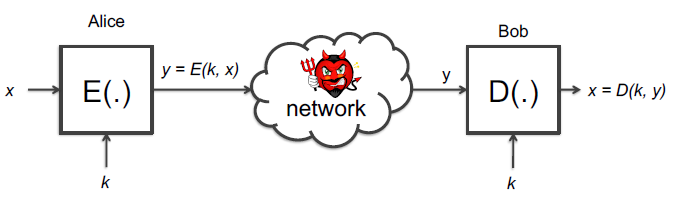
\includegraphics{./immagini/modello.png} 
    
    \subsubsection{Definizione di Cifrario}
        Un cifrario, o schema di cifratura, è defito su una tripletta composta da (K,P,C) usata nelle funzioni di (Gen,Enc,Dec) definite con questi domini: 
         \begin{align}
            &Gen: Z^+ \to K funzione generatrice di chiavi\\  
            &Enc: P \times K \to C  funzione di cifratura\\
            &Dec : C \times K \to P funzione di decifratura\\
            &x \in P , y \in C , k \in K\\
            &y = Enc(k,x)\\
            &x = Dec(k,y)
        \end{align}
        \paragraph{Proprieta di cifratura}
            La cifratura deve anche rispettare le seguenti proprieta: 
            \begin{description}
                 \item[Correttezza]: $\forall p \in P \land k \in K, \exists Dec(k,Enc(k,p)) = p$
                 \item[Sicurezza]:  Un cifrario simmetrico è sicuro $\iff \forall (p,c), p \in P \land c \in C  \Rightarrow$ 
                 \begin{itemize}
                            \item dato \textit{c} ciphertext, è "difficile" determinare \textit{p} plaintext senza conoscere la chiave \textit{k}, e viceversa
                            \item è "difficile" determinare \textit{k} chiave, ammenoche non sia stata già usata una volta
               \end{itemize}
            \end{description}

        \paragraph{Esempio : Sostituzione monoalfabetca} 
            Vediamo quindi un tipo di cifratura a sostituzione, dove la chiave è la permutazione dell' alfabeto. L' algoritmo prevede la sostituzione delle lettere della parola con le corrispondenti dell' alfabeto shiftato, e per decriptare si usa l' algoritmo al contrario. Le chiavi quindi possono essere circa  26! cioè circa $4\cdot10^26$, quindi tentare un attacco a forza bruta non è possibile, ma è possibile applicare tecniche di Crittoanalisi analizzando alcune proprietà che riguardano i linguaggi come : la frequenza delle lettere, la generalizzazione delle coppie e triple di lettere, la frequenza delle parole corte se sono identificati i separatori.  
    \subsubsection{Crittoanalisi}        
            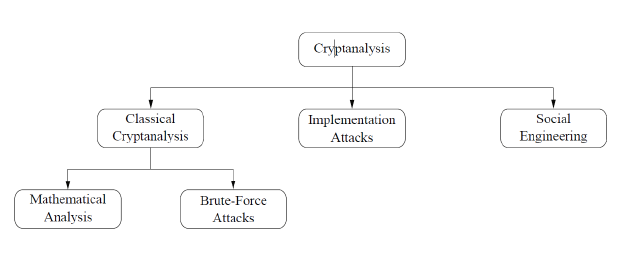
\includegraphics{./immagini/crittoanalisi.png}
               
          \paragraph{Complessità dell'attacco} Viene definito da:
                \begin{description}
                    \item[Complessità dei Dati:] Numero previsto di unità dei dati in ingresso richiesti.
                    \item[Complessità di Storage:] Numero previsto delle unità di storage richiesti.
                    \item[Complessità di Elaborazione:] Numero previsto di operazioni richiesti per processare i dati in input o/e per riempire la memoria con dati.
                \end{description}
            
           \paragraph{Tipi di attacco} Si possono classificare in:
               
                \begin{itemize}
                    \item Ciphertext-only attack
                    \item Known-plaintext attack
                    \item Chosen-plaintext attack (CPA)
                \end{itemize}
                Se un metodo è sicuro contro i CPA, allora è sicuro anche contro gli altri.
            \paragraph{Principi di Kerchoff}

            \begin{description}
                \item[Massima di Kerckhoffs] Un sistema crittografico dovrebbe rimanere sicuro anche se tutto del sistema, tranne la chiave, è di pubblico dominio.
                
                \item[Massima di Shannon] Il nemico conosce il sistema.
                
                \item[Massima di Bruce Schneier] Meno e più semplici sono i segreti da custodire per garantire la sicurezza del sistema, più facile sarà mantenerne la sicurezza.
            \end{description}

            \textbf{Consigli per mantenera la sicurezza facile}
            \begin{itemize}
                \item Le chiavi sono piccoli segreti.
                \item Conservare piccoli segreti è più facile che conservare grandi segreti.
                \item Sostituire piccoli segreti, una volta eventualmente compromessi, è più facile (ed economico) che sostituire grandi segreti.
            \end{itemize}

        \subsubsection{Esempi di cifrari} 
            \paragraph{Cifrario di cesare}

            Siano $PT$, $CT$ e $K$ elementi dell'anello $Z_{26}$.

            \begin{itemize}
                \item \textbf{Cifratura (Encryption):} \[
                y = x + k \mod 26
                \]
                
                \item \textbf{Decifratura (Decryption):} \[
                x = y - k \mod 26
                \]
                
                \item \textbf{Esempio:}
                \begin{itemize}
                    \item Testo in chiaro (Plaintext, $x$): ``\texttt{ATTACK}'' $\Rightarrow$ \[x = (0, 19, 19, 0, 2, 10)\]
                    \item Chiave ($k$): \[k = 17\]
                    \item Testo cifrato (Ciphertext, $y$): \[
                    y = (0+17, 19+17, 19+17, 0+17, 2+17, 10+17) \mod 26 = (17, 10, 10, 17, 19, 1)
                    \]
                    \item Risultato: ``\texttt{RKKRTB}''
                \end{itemize}
            \end{itemize}

            \paragraph{Cifrario Affine}

            \subparagraph{Definizione}

Siano $a, b, x, y \in Z_{26}$.

\begin{itemize}
    \item \textbf{Cifratura (Encryption):}
    \[
    y = a \cdot x + b \mod 26
    \]
    
    \item \textbf{Decifratura (Decryption):}
    \[
    x = a^{-1} \cdot (y - b) \mod 26
    \]
    
    \item La chiave è $k = (a, b)$, con $\gcd(a, 26) = 1$
    
    \item \textbf{Esempio:}
    \begin{itemize}
        \item Testo in chiaro (Plaintext): ``\texttt{ATTACK}'' $\Rightarrow (0, 19, 19, 0, 2, 10)$
        \item Chiave $k = (9, 13)$
        \item Cifratura:
        \[
        y = (9 \cdot x + 13) \mod 26
        \]
        \[
        y = (13, 2, 2, 13, 5, 25)
        \]
        \item Testo cifrato (Ciphertext): ``\texttt{NCCNFZ}''
    \end{itemize}
\end{itemize}

\subparagraph{Calcolo dello spazio delle chiavi}

Lo spazio delle chiavi si calcola come:
\[
\text{Spazio delle chiavi} = N_a \cdot N_b
\]

Dove:
\begin{itemize}
    \item $N_a$ è il numero di valori possibili di $a$ tali che $\gcd(a, 26) = 1$. \\
    In questo caso: $N_a = 12$
    \item $N_b$ è il numero dei possibili valori di shift $b$ in $Z_{26}$. \\
    Quindi: $N_b = 26$
\end{itemize}

Pertanto, lo spazio delle chiavi è:
\[
12 \cdot 26 = 312
\]


\section{Cifrario Perfetto}
  \subsection{Introduzione}
            Nel contesto della sicurezza crittografica, si considera un attaccante con la capacità di condurre un \textit{ciphertext-only attack}, ovvero un attacco in cui l'unica informazione disponibile è il testo cifrato.

            \paragraph{Requisiti di sicurezza}
                Un cifrario è considerato sicuro se soddisfa i seguenti requisiti:
            \begin{itemize}
                \item L'attaccante non è in grado di recuperare la chiave segreta.
                \item L'attaccante non è in grado di risalire al testo in chiaro (plaintext).
                \end{itemize}

            \paragraph{Intuizione di un cifrario perfettamente sicuro}
                L'idea alla base di un cifrario perfettamente sicuro è che, indipendentemente da qualsiasi informazione pregressa che l'attaccante possa avere sul testo in chiaro, il testo cifrato non deve fornire alcuna informazione aggiuntiva su di esso.
  \subsection{Approccio Probabilistico}
   Nel contesto della crittografia, il messaggio $M$ viene modellato come una variabile aleatoria, secondo una distribuzione di probabilità detta \textit{distribuzione del plaintext}. Ad esempio, si potrebbe avere:

  \begin{itemize}
      \item $\Pr[M = \text{``attack today''}] = 0.7$
      \item $\Pr[M = \text{``don't attack''}] = 0.3$
  \end{itemize}
  
  Queste probabilità rappresentano la \textit{conoscenza a priori} che un attaccante potrebbe avere riguardo al contenuto del messaggio.
  
  Il generatore di chiavi $\text{Gen}()$ definisce una distribuzione di probabilità sulla chiave $K$, ovvero:
  \[
  \Pr[K = k] = \Pr[k \leftarrow \text{Gen}()]
  \]
  Le variabili aleatorie $M$ (messaggio) e $K$ (chiave) si assumono indipendenti.
  
  \paragraph{Processo di generazione del ciphertext}
  \begin{enumerate}
      \item Si sceglie un messaggio $m$ secondo la distribuzione di $M$.
      \item Si genera una chiave $k$ da $\text{Gen}()$.
      \item Si calcola il testo cifrato $c \leftarrow E_k(m)$.
  \end{enumerate}
  
  Il testo cifrato $C$ risultante è anch'esso una variabile aleatoria, e il processo di cifratura definisce una distribuzione di probabilità indotta su $C$.

  \paragraph{Segretezza Perfetta}

  La \textit{segretezza perfetta} è un concetto fondamentale introdotto da Claude Shannon nel 1949. In modo informale, si riferisce alla condizione in cui il testo cifrato non rivela alcuna informazione sul testo in chiaro. Formalizziamo l'idea di ``informazione sul plaintext'' in termini di distribuzione di probabilità.
  
  Un sistema di cifratura gode di segretezza perfetta se, per ogni messaggio $m \in M$ e ogni testo cifrato $c \in C$ tale che $\Pr[C = c] > 0$, vale la seguente uguaglianza:
  \[
  \Pr[M = m \mid C = c] = \Pr[M = m]
  \]
  Questo implica che la probabilità a posteriori che un messaggio sia $m$, dato il testo cifrato $c$, è uguale alla probabilità a priori che il messaggio fosse $m$: osservare il testo cifrato non fornisce alcuna informazione aggiuntiva.
  
  Una formulazione equivalente della segretezza perfetta è la seguente:
  \[
  \forall m, m' \in M, \forall c \in C, \quad \Pr[E_k(m) = c] = \Pr[E_k(m') = c]
  \]
  In altre parole, la distribuzione del testo cifrato è indipendente dal messaggio originale. La distribuzione a priori del plaintext (prima di osservare il ciphertext) e quella a posteriori (dopo aver osservato il ciphertext) devono coincidere.
  
  \subsubsection{Teorema di Shannon}

  \paragraph{Teorema di Shannon}
  \begin{itemize}
      \item In un cifrario perfetto, $|K| \geq |M|$
      \item Ovvero, il numero di chiavi non può essere inferiore al numero di messaggi
  \end{itemize}
  
  \paragraph{Dimostrazione (per assurdo):}
  \begin{enumerate}
      \item Supponiamo che $|K| < |M|$
      \item Deve valere $|C| \geq |M|$, altrimenti il cifrario non è invertibile
      \item Quindi, $|C| > |K|$
      \item Sia $m \in M$ tale che $\Pr[M = m] \neq 0$; si calcoli $c_i \leftarrow E(k_i, m)$ per ogni $k_i \in K$
      \item Per il punto (3), esiste almeno un $c$ tale che $c \neq c_i$ per ogni $k_i \in K$
      \item Allora $\Pr[M = m \mid C = c] = 0$, che è diverso da $\Pr[M = m]$, contraddicendo la definizione di cifrario perfetto
  \end{enumerate}
  
  \paragraph{Fatto.} Sia $\Pi = (\text{Gen}, \text{Enc}, \text{Dec})$ uno schema di cifratura con $|M| = |K| = |C|$. Lo schema è perfettamente sicuro se e solo se:
  \begin{enumerate}
      \item  $\forall k \in K$ è scelto con probabilità uniforme $1/|K|$ da Gen
      \item  $\forall m \in M \land c \in C, \exists! k \in K : E_k(m) = c$
  \end{enumerate}
  
  \paragraph{Nota:}
  \begin{itemize}
      \item La condizione 1 è facile da verificare
      \item La condizione 2 non richiede il calcolo di probabilità
  \end{itemize}
  
  \subsubsection{Sicurezza incondizionata}
  La perfetta segretezza è equivalente alla sicurezza incondizionata. In questo modello, si assume che un avversario disponga di risorse computazionali illimitate. L'osservazione del testo cifrato non fornisce quindi alcuna informazione utile all'avversario riguardo al messaggio originale.
  
  \paragraph{Condizioni necessarie}
  \begin{itemize}
      \item I bit della chiave devono essere scelti in modo veramente casuale
      \item La lunghezza della chiave deve essere maggiore o uguale alla lunghezza del messaggio (secondo il teorema di Shannon)
  \end{itemize}
  
  \subsubsection{Indistinguibilità perfetta}
  Sia $\Pi = (G, E, D)$ uno schema di cifratura definito su insiemi $K$, $M$, $C$.
  
  $\Pi$ ha \emph{indistinguibilità perfetta} se e solo se:
  \[
  \forall m_1, m_2 \in M,\ |m_1| = |m_2|,\ \forall c \in C,\ \text{con } k \leftarrow G \text{ uniforme}:
  \quad \Pr[E(k, m_1) = c] = \Pr[E(k, m_2) = c]
  \]
  
  \subparagraph{Fatto}
  $\Pi$ ha indistinguibilità perfetta $\iff$ $\Pi$ è perfettamente sicuro.
  
            
    \subsection{One-Time Pad}
    Il \textit{One-Time Pad} è un sistema di cifratura brevettato da Vernam nel 1917, ma il suo principio era già noto circa 35 anni prima. È stato dimostrato perfettamente sicuro da Claude Shannon nel 1949. Un'applicazione celebre di questo metodo è il collegamento diretto e sicuro tra Mosca e Washington, noto come ``telefono rosso'', che in realtà non era un telefono ma un sistema di comunicazione sicura basato su teletype, fax e collegamenti informatici criptati.

    \subsubsection{Concetti preliminari}
    
    Il \textit{One-Time Pad} si basa sull'operazione logica \texttt{XOR} (OR esclusivo), definita dalla seguente regola:
    \[
    z = x \oplus y = (x + y) \mod 2
    \]
    
    \paragraph{Assunzioni}
    
    Sia $x \in \{0,1\}^t$ un messaggio binario di $t$ bit e $k \in \{0,1\}^t$ una chiave di pari lunghezza, i cui bit sono scelti in modo completamente casuale.
    
    \paragraph{Cifratura}
    
    Per ogni $i \in [1, \dots, t]$, il bit cifrato $y_i$ si ottiene come:
    \[
    y_i = m_i \oplus k_i \quad \text{ovvero} \quad y_i = (m_i + k_i) \mod 2
    \]
    
    \paragraph{Decifratura}
    
    Per ogni $i \in [1, \dots, t]$, si recupera il messaggio originale come:
    \[
    x_i = c_i \oplus k_i \quad \text{ovvero} \quad x_i = (y_i + k_i) \mod 2
    \]
    
    La proprietà di consistenza del sistema (cioè $x_i = m_i$ dopo cifratura e decifratura) è facilmente dimostrabile grazie alla simmetria dell'operazione \texttt{XOR}.
    
    \paragraph{XOR come buona funzione di cifratura}

\textbf{Teorema.} Sia $X$ una variabile aleatoria su $\{0,1\}^n$ e $K$ una variabile aleatoria indipendente e uniformemente distribuita su $\{0,1\}^n$. Allora $Y = X \oplus K$ è uniformemente distribuita su $\{0,1\}^n$.

\paragraph{Dimostrazione (caso $n = 1$)}
Siano $\Pr[X = 0] = X_0$ e $\Pr[X = 1] = X_1$, con $X_0 + X_1 = 1$.\\
Allora:
\[
\Pr[Y = 0] = \Pr[X = 0 \land K = 0] + \Pr[X = 1 \land K = 1] = X_0 \cdot 0.5 + X_1 \cdot 0.5 = 0.5 (X_0 + X_1) = 0.5
\]
e analogamente $\Pr[Y = 1] = 0.5$. Quindi $Y$ è uniforme.

\paragraph{Pro e contro dell'One-Time Pad}

L'One-Time Pad (OTP) è un sistema crittografico estremamente sicuro, ma presenta anche importanti limitazioni pratiche.

\subparagraph{Pro}
\begin{itemize}
    \item \textbf{Sicurezza incondizionata}: un sistema è detto incondizionatamente sicuro (o sicuro dal punto di vista dell'informazione) se non può essere violato nemmeno disponendo di risorse computazionali illimitate.
    \item \textbf{Ottimalità}: l'OTP è ottimale in quanto ogni chiave cifra un solo messaggio in un solo testo cifrato. Vale che $|M| = |K| = |C|$.
    \item \textbf{Efficienza}: la cifratura e decifratura sono operazioni estremamente veloci, basate su un semplice XOR bit a bit.
\end{itemize}

\subparagraph{Contro}
\begin{itemize}
    \item \textbf{Chiavi lunghe}: la chiave deve essere lunga quanto il messaggio, il che rende il sistema poco pratico. In generale, $|K| \geq |M|$.
    \item \textbf{Riutilizzo della chiave proibito}: la chiave deve essere usata una sola volta. Il riutilizzo (due-time pad) compromette la sicurezza. Se $C_1 = M_1 \oplus K$ e $C_2 = M_2 \oplus K$, allora $C_1 \oplus C_2 = M_1 \oplus M_2$.
    \item \textbf{Attacchi con testo in chiaro noto}: conoscendo una coppia $(m, c)$, si può ricavare direttamente la chiave $k = m \oplus c$.
    \item \textbf{Malleabilità}: il sistema è malleabile, cioè modifiche al testo cifrato si riflettono in modo prevedibile sul testo in chiaro senza essere rilevate.
\end{itemize}

\paragraph{Segretezza perfetta dell’One-Time Pad}

\textbf{Teorema.} Il cifrario One-Time Pad soddisfa la segretezza perfetta.

\paragraph{Dimostrazione}
\begin{enumerate}
    \item Per definizione di probabilità condizionata (legge di Bayes):
    \[
    \Pr[M = m \mid C = c] = \frac{\Pr[C = c \mid M = m] \cdot \Pr[M = m]}{\Pr[C = c]}
    \]
    \item Calcoliamo $\Pr[C = c]$ usando la legge della probabilità totale:
    \[
    \Pr[C = c] = \sum_i \Pr[C = c \mid M = m_i] \cdot \Pr[M = m_i] = \sum_i \Pr[K = c \oplus m_i] \cdot \Pr[M = m_i]
    \]
    Poiché $K$ è uniforme, $\Pr[K = c \oplus m_i] = 2^{-k}$:
    \[
    \Pr[C = c] = \sum_i 2^{-k} \cdot \Pr[M = m_i] = 2^{-k}
    \]
    \item Sostituendo nella formula iniziale:
    \[
    \Pr[M = m \mid C = c] = \frac{2^{-k} \cdot \Pr[M = m]}{2^{-k}} = \Pr[M = m]
    \]
\end{enumerate}

Quindi il testo cifrato non rivela alcuna informazione aggiuntiva sul messaggio: l'OTP ha segretezza perfetta.
\paragraph{Malleabilità}

Un sistema crittografico si dice \textit{malleabile} se un attaccante è in grado di trasformare un testo cifrato in un altro testo cifrato tale che il corrispondente testo in chiaro subisce una trasformazione prevedibile. In questo scenario, l’attaccante non decifra direttamente il messaggio, ma riesce comunque a manipolarlo in modo controllato e coerente, ottenendo un effetto noto sul contenuto in chiaro.

\paragraph{Sulla malleabilità dell'OTP}

Un esempio di attacco contro l'integrità di un sistema OTP si verifica quando un attaccante intercetta il testo cifrato e lo manipola in modo che il testo in chiaro risultante sia una versione trasformata ma prevedibile del messaggio originale.

\subparagraph{Attacco contro l'integrità}
\begin{itemize}
    \item Alice invia a Bob il testo cifrato $c = p \oplus k$, dove $p$ è il messaggio e $k$ è la chiave.
    \item L'avversario intercetta $c$ e trasmette a Bob un testo cifrato modificato $c' = c \oplus r$, dove $r$ è chiamato perturbazione.
    \item Bob riceve $c'$ e lo decifra: $p' = c' \oplus k = (c \oplus r) \oplus k = (p \oplus k) \oplus r \oplus k = p \oplus r$, ottenendo così $p' = p \oplus r$.
    \item La perturbazione $r$ passa inosservata e ha un impatto prevedibile sul testo in chiaro.
\end{itemize}



\textbf{RIGUARDARE GLI ESERCIZI SULLA PROBABILITÃ Slide 1.01}



\section{Stream Chipers}
    \subsubsection{Come faccio un OTP in pratica?}
    L'idea è usare, al posto di una chiave di stream completamente casuale, una chiave pseudo-casuale utilizzando uno \textit{Pseudo Random Generator} G che è una funzione efficiente e deterministica, che utilizza un \textit{seed} per generare poi un valore pseudo-casuale con 
    \[G: \{0,1\}^s(\text{Spazio del seed}) \rightarrow \{0,1\}^n (\text{spazio della Chiave}), n (\text{dimensioni della chiave}) \gg s (\text{dimensioni del seed})\]
    si ha quindi poi come funzione di criptazione $y = G(k) \oplus x$  e come funzione di decriptazione $x = G(k) \oplus y$ con \textit(k) che viene utilizzata come seed della funzione. 
    Si viene però a creare un problema ovvero il numero di chiavi $|k|$ è minore del numero di messaggi $|m|$, violando cosi il principio si Shannon. 
    La sicurezza dipenderà dallo specifico Generatore Pseudo-Casuale (PRG, in inglese Pseudo-Random Generator). È fondamentale che un PRG appaia casuale, ovvero che sia indistinguibile da un vero generatore casuale (TRG, True Random Generator) per un avversario con capacità limitate.

Deve essere computazionalmente irrealizzabile distinguere l'output di un PRG da quello di un TRG. Questo concetto introduce una nuova definizione di sicurezza: la \textbf{sicurezza computazionale}.

\paragraph{Sicurezza computazionale}
Un cifrario si dice \textbf{computazionalmente sicuro} (in modo pratico) se il livello percepito di computazione necessario per violarlo, utilizzando il miglior attacco noto, supera, con un buon margine, le risorse computazionali dell’avversario ipotizzato.

In questa prospettiva, l'avversario viene considerato come avente una potenza di calcolo limitata. Tuttavia, è fondamentale porsi la domanda: qual è il miglior attacco conosciuto? Anche se si conosce un limite inferiore della complessità di un attacco, non si può escludere che esistano attacchi più potenti e non ancora scoperti.

Pertanto, la miglior strategia attuale è progettare sistemi crittografici assumendo che siano \textbf{computazionalmente sicuri}.

\paragraph{Imprevedibilità del PRG}
Un PRG, oltre ad avere buone proprietà statistiche, deve essere \textbf{imprevedibile}. Se un PRG risulta prevedibile, allora un cifrario a flusso che lo utilizza non può essere considerato sicuro.

Supponiamo che un avversario sia in grado di determinare un prefisso della sequenza generata \( x \). In tal caso, egli può calcolare un prefisso del keystream (flusso di chiavi). Se la funzione di generazione \( G \) è prevedibile, l’avversario potrà calcolare anche il resto del keystream, riuscendo quindi a decifrare il messaggio cifrato \( y \).

\paragraph{Imprevedibilità in avanti}
L’\textbf{imprevedibilità in avanti} richiede che, se il seme iniziale (seed) non è noto, allora il prossimo bit della sequenza generata deve essere imprevedibile, indipendentemente dalla conoscenza di un qualsiasi prefisso della sequenza.

\paragraph{Imprevedibilità all’indietro}
L’\textbf{imprevedibilità all’indietro} implica che non deve essere possibile risalire al seme a partire dalla conoscenza di una qualsiasi porzione della sequenza generata.

In sintesi, anche se una sequenza appare o si comporta come casuale, non deve essere possibile prevedere né i bit successivi né risalire al seme che ha generato la sequenza.
 
\begin{figure}[h]
    \centering
    \includegraphics{./immagini/TRBG.png}
    \caption{Schema di generazione di una sequenza pseudocasuale. 
    Un processo casuale vero (true random process) genera una sequenza casuale attraverso una fase di digitalizzazione. 
    Questa sequenza casuale può essere utilizzata come \textit{seed} per un generatore pseudocasuale (PRBG, \textit{Pseudorandom Bit Generator}),
    il quale produce una sequenza pseudocasuale. Il contesto applicativo può influenzare il comportamento del PRBG.}
\end{figure}

\subsection{State of Art e Casi studio}
    \subsubsection{WEP}
    Nel protocollo 802.11b WEP, viene utilizzata una chiave segreta $k$ di lunghezza fissa pari a 104 bit. Per ogni nuovo messaggio viene scelto un nuovo IV (Initialization Vector), lungo 24 bit. L'uso dell'IV serve ad evitare l'utilizzo dello stesso keystream per due messaggi diversi, condizione nota come two-time pad (2TP), che comprometterebbe la sicurezza.

La procedura di cifratura prevede che il messaggio $m$ venga concatenato al suo checksum (calcolato tramite una funzione CRC), e poi cifrato utilizzando un keystream generato da una funzione pseudocasuale, la quale prende come input la concatenazione dell'IV e della chiave $k$, ovvero $PRG(IV || k)$. Il pacchetto trasmesso contiene l'IV in chiaro seguito dal ciphertext.

Tuttavia, la limitata lunghezza dell'IV (24 bit) implica che, dopo circa $2^{24} \approx 16$ milioni di frame trasmessi, è probabile che si verifichino ripetizioni dell'IV. Inoltre, su alcune schede 802.11, l'IV viene semplicemente incrementato frame dopo frame (ad esempio, chiave per il frame \#1: $1||k$, per il frame \#2: $2||k$, per il frame \#3: $3||k$, e così via), e in alcuni casi, dopo un ciclo di spegnimento e riaccensione, l'IV viene azzerato. Queste pratiche generano chiavi strettamente correlate tra loro, anziché casuali, riducendo drasticamente la sicurezza del sistema.

A causa di queste debolezze, nel 2001 Fluhrer, Mantin e Shamir (FMS) hanno dimostrato che è possibile recuperare la chiave $k$ osservando circa $10^6$ frame cifrati. Con miglioramenti successivi all'attacco, oggi bastano circa 40.000 frame per compromettere la chiave. È quindi fondamentale evitare la generazione di chiavi correlate e preferire costruzioni più sicure, dove ogni frame dispone di una chiave pseudocasuale indipendente.


\subsubsection{Linear Feedback Shift Register (LFSR)}
Il Linear Feedback Shift Register (LFSR) è un circuito digitale utilizzato per generare sequenze di bit pseudo-casuali. È composto da un registro a scorrimento, costituito da celle di memoria (flip-flop), e da una logica di retroazione che combina i valori presenti nelle celle attraverso operazioni di somma modulo 2 (XOR).
\includegraphics{./immagini/LFSR.png}
\subparagraph{Funzionamento}
Ad ogni impulso di clock, il contenuto delle celle viene fatto scorrere verso destra e il nuovo bit da inserire nella cella più a sinistra viene calcolato come combinazione lineare dei bit precedenti, in base a specifici coefficienti di retroazione $p_j$. Se un coefficiente $p_j$ è pari a 1, significa che il bit corrispondente partecipa al calcolo della retroazione; se è 0, non partecipa. Formalmente, il nuovo bit generato $s_{i+m}$ è calcolato come:
\[
s_{i+m} = \sum_{j=0}^{m-1} p_j \cdot s_{i+j} \mod 2
\]
dove $m$ è il grado del registro, ovvero il numero di celle di memoria.

\paragraph{Proprietà degli LFSR}
\subparagraph{Seed}
Il \emph{seed} è lo stato iniziale del registro. È fondamentale che il seed non sia tutto composto da zeri, poiché in tal caso l'LFSR rimarrebbe bloccato permanentemente nello stato nullo, senza generare alcuna sequenza utile.

\subparagraph{Grado}
Il grado dell'LFSR è definito come il numero di celle di memoria presenti nel registro. Ad esempio, se sono presenti 8 flip-flop, si dice che l'LFSR ha grado 8.

\subparagraph{Periodicità}
La sequenza di bit generata da un LFSR è \emph{periodica}. Questo significa che, dopo un certo numero di cicli, la sequenza di stati del registro si ripete identicamente.

\subparagraph{Massima lunghezza}
Un LFSR può generare una sequenza di lunghezza massima pari a $2^m - 1$, dove $m$ è il grado del registro. Questa proprietà è garantita solo se i coefficienti di retroazione sono scelti opportunamente. In particolare, esiste un teorema che afferma che la lunghezza massima della sequenza generata da un LFSR di grado $m$ è $2^m - 1$. Gli LFSR che raggiungono questa lunghezza massima sono detti \emph{maximum-length LFSR} e possono essere facilmente costruiti con una scelta adeguata dei tap di retroazione.

\paragraph{Pro e contro degli LFSR}
Gli LFSR presentano numerosi vantaggi, ma anche alcune debolezze significative che è importante considerare attentamente.

\subparagraph{Vantaggi}
Uno dei principali punti di forza degli LFSR è che producono sequenze di bit con ottime proprietà statistiche. Le sequenze generate sono bilanciate (hanno circa lo stesso numero di 0 e di 1) e hanno buone proprietà di autocorrelazione, il che li rende ideali per applicazioni in ambito di crittografia e comunicazioni digitali, come la generazione di chiavi o il riempimento di canali.

\subparagraph{Svantaggi}
Nonostante le buone proprietà statistiche, gli LFSR sono strutture \emph{periodiche}, cioè la sequenza generata si ripete dopo un numero finito di passi. Inoltre, sono dispositivi \emph{lineari}, e questa linearità li rende vulnerabili ad attacchi crittografici sofisticati.

\paragraph{Attacco Known-Plaintext contro LFSR}
Gli LFSR sono particolarmente vulnerabili a un tipo di attacco chiamato \emph{Known-Plaintext Attack}. Questo attacco si articola in tre fasi principali:
\begin{enumerate}
    \item L'avversario raccoglie almeno $2m$ coppie di testo in chiaro ($pt$) e testo cifrato ($ct$), dove $m$ è il grado dell'LFSR.
    \item Utilizzando queste coppie, l'avversario è in grado di determinare un prefisso della sequenza $s_i$ generata dall'LFSR.
    \item Infine, l'avversario risolve un sistema di $m$ equazioni lineari in $m$ incognite per determinare i coefficienti di retroazione $p_j$. Una volta ottenuti questi coefficienti, può ricostruire completamente l'LFSR e prevedere tutta la sequenza futura.
\end{enumerate}

\paragraph{Gli LFSR devono essere abbandonati?}
Nonostante le vulnerabilità individuate, gli LFSR non devono essere necessariamente scartati. Una soluzione consiste nell'utilizzare una combinazione \emph{non lineare} di più LFSR per costruire cifrari robusti. Un esempio tipico è quello di utilizzare operazioni logiche come l'AND tra i segnali di uscita di diversi LFSR, aumentando così la complessità e la sicurezza del sistema risultante. Un esempio concreto di questo approccio è il cifrario Trivium, progettato nel 2003, che combina più registri a scorrimento tramite operazioni non lineari per ottenere una robustezza crittografica elevata.

\paragraph{State of the Art}
Nel panorama attuale della cifratura a flusso, esistono differenti approcci, principalmente suddivisi tra soluzioni orientate al software e soluzioni orientate all'hardware.

\subparagraph{Software Oriented}
Tra i cifrari a flusso orientati al software si annoverano algoritmi come RC4 e SEAL. Entrambi sono stati ampiamente studiati e analizzati dalla comunità scientifica, risultando generalmente sicuri, anche se l'uso di RC4 oggi è sconsigliato in nuovi progetti a causa di alcune vulnerabilità emerse nel tempo.

\subparagraph{Hardware Oriented}
Per quanto riguarda le implementazioni hardware, molte soluzioni si basano su registri a scorrimento con retroazione lineare (LFSR). Tuttavia, molte di queste soluzioni sono state compromesse nel tempo. Un esempio emblematico è dato dagli algoritmi di cifratura GSM, A5/1 e A5/2. A5/1 era originariamente un algoritmo segreto, ma è stato successivamente decifrato attraverso operazioni di reverse engineering. A5/2, invece, presenta vulnerabilità ancora più gravi e può essere attaccato in tempi relativamente brevi. Attualmente, né A5/1 né A5/2 sono raccomandati per garantire comunicazioni sicure. A5/3, noto anche come KASUMI, rappresenta un miglioramento significativo: è infatti un cifrario a blocchi, e non più un puro cifrario a flusso.

\subparagraph{eSTREAM Project}
Per migliorare la situazione dei cifrari a flusso, è stato lanciato il progetto eSTREAM, parte della ECRYPT Network of Excellence. L'obiettivo era selezionare cifrari moderni e sicuri adatti a diverse applicazioni. Il progetto ha raccolto 34 candidati, suddivisi in due profili:
\begin{itemize}
    \item \textbf{Profilo 1}: Cifrari a flusso destinati ad applicazioni software con requisiti di alta velocità di trasmissione. Tra i principali candidati troviamo HC-128, Rabbit, Salsa20/12 e SOSEMANUK.
    \item \textbf{Profilo 2}: Cifrari a flusso progettati per applicazioni hardware con risorse limitate. In questo contesto si distinguono Grain v1, MICKEY v2 e Trivium.
\end{itemize}

\subparagraph{Performance dei cifrari eSTREAM}
I risultati ottenuti nel progetto eSTREAM hanno mostrato performance molto promettenti. Su una piattaforma AMD Opteron da 2.2 GHz con sistema operativo Linux, sono state misurate le seguenti velocità:
\begin{itemize}
    \item RC4: 126 Mb/s
    \item Salsa20/12: 643 Mb/s
    \item SOSEMANUK: 727 Mb/s
\end{itemize}
Questi risultati evidenziano come i cifrari di nuova generazione riescano a superare di gran lunga le prestazioni di RC4, offrendo allo stesso tempo una maggiore sicurezza.

\subsection{CONTENT SCRAMBLING SYSTEM (CSS)}

Il Content Scrambling System (CSS) è un sistema di cifratura utilizzato per proteggere i contenuti, ad esempio nei DVD. Alla base del sistema ci sono due LFSR (Linear Feedback Shift Registers) il cui stato iniziale è determinato da un \emph{seed} o chiave di 5 byte, pari a 80 bit.

\paragraph{Funzionamento di ogni round}
Durante ogni round di generazione del flusso di chiavi, si eseguono 8 cicli di clock. In ogni ciclo, ciascun LFSR produce 8 bit di output. Gli output dei due LFSR vengono poi sommati modulo 256 per ottenere un byte di keystream. Per semplicità, il bit di riporto generato dall'addizione viene trascurato.

\paragraph{Vulnerabilità}
Il CSS risulta estremamente vulnerabile: può essere rotto con una complessità di appena $2^{17}$ operazioni, un valore molto inferiore rispetto alla complessità attesa di $2^{40}$.

\paragraph{Attacco Known Plaintext}
L'attacco sfrutta il fatto che un prefisso del filmato, pari a circa 20 byte, è noto in chiaro (ad esempio, i primi 20 byte di un file MPEG). Questo consente di ricavare direttamente un prefisso corrispondente del keystream. Conoscendo questa parte iniziale del keystream, diventa possibile ricostruire il seed iniziale.

\paragraph{Algoritmo di attacco}
L'attacco procede come segue:
\begin{enumerate}
    \item Si considerano tutte le possibili configurazioni iniziali di LFSR17, pari a $2^{17}$ possibilità.
    \item Per ogni configurazione, si esegue LFSR17 per ottenere i primi 20 byte di output.
    \item Si sottrae questo output dal prefisso noto del keystream per ottenere un candidato output di LFSR25.
    \item Si verifica se il candidato è coerente con il funzionamento di LFSR25:
    \begin{itemize}
        \item Se è coerente, si è trovato il corretto stato iniziale di entrambi gli LFSR e l'algoritmo termina.
        \item Altrimenti, si passa alla configurazione successiva di LFSR17 e si ripete il processo.
    \end{itemize}
\end{enumerate}
Una volta individuato il seed corretto, è possibile generare l'intero output del CSS. La complessità massima dell'attacco è quella di testare tutte le possibili configurazioni iniziali di LFSR17, ovvero $2^{17}$ tentativi.


\subsection{RBG}
\subsubsection{Definizione}

Un \textbf{Random Bit Generator} (RBG) è un generatore che produce una sequenza di bit statisticamente indipendenti e non polarizzati.

\paragraph{Indipendenza statistica}
L'indipendenza statistica implica che la probabilità di emissione di un valore di bit (0 oppure 1) non dipende dai bit precedentemente generati. In altre parole, ogni bit è generato senza alcuna influenza dai bit passati.

\paragraph{Assenza di polarizzazione}
L'assenza di polarizzazione (unbiased) significa che la probabilità di generare un bit 0 oppure 1 è esattamente pari a \( 0.5 \). Ogni bit ha quindi la stessa probabilità di assumere uno dei due valori possibili.

\paragraph{Random Number Generator (RNG)}
I \textbf{Random Number Generator} (RNG) possono essere utilizzati per generare numeri casuali distribuiti uniformemente. Un numero casuale nell’intervallo \([0, n]\) può essere ottenuto generando una sequenza casuale di bit di lunghezza \( \lceil \log_2(n+1) \rceil \) e convertendola in un intero.

Se il numero risultante supera \( n \), una possibile soluzione consiste nello scartarlo e nel generare una nuova sequenza casuale di bit, ripetendo il processo fino a ottenere un numero valido.

\paragraph{Classi di RBG}
Esistono diverse classi di Random Bit Generator:
\begin{itemize}
    \item \textbf{True Random Bit Generator (TRBG)}: generatori di bit veramente casuali, basati su fenomeni fisici imprevedibili.
    \item \textbf{Pseudorandom Bit Generator (PRBG)}: generatori di bit pseudocasuali, che producono sequenze apparentemente casuali ma deterministiche a partire da un seme iniziale.
    \item \textbf{Cryptographically Secure Pseudorandom Bit Generator (CSPRBG)}: una particolare categoria di PRBG progettata per soddisfare criteri di sicurezza crittografica, rendendo impraticabile per un avversario prevedere parti della sequenza o risalire al seme.
\end{itemize}


\subsubsection{True Random Bit Generators (TRBG) Hardware-based}

I \textbf{True Random Bit Generators} (TRBG) hardware-based si basano su fenomeni fisici che sono naturalmente casuali. Questi generatori sfruttano eventi o processi fisici imprevedibili per produrre sequenze di bit che non possono essere riprodotte in modo deterministico.

\paragraph{Fenomeni fisici utilizzati}
Ecco alcuni esempi di fenomeni fisici che possono essere utilizzati per generare casualità:
\begin{itemize}
    \item \textbf{Tempo trascorso tra l'emissione di particelle durante il decadimento radioattivo}: Il decadimento radioattivo è un processo fondamentale per la generazione di numeri casuali, in quanto è intrinsecamente casuale e non può essere previsto.
    \item \textbf{Rumore termico da un diodo semiconduttore o da una resistenza}: Il rumore termico è una fluttuazione casuale che si verifica a livello microscopico nei semiconduttori e che può essere misurato per generare numeri casuali.
    \item \textbf{Instabilità di frequenza di un oscillatore a libera corsa}: Gli oscillatori, come quelli in un circuito elettronico, possono mostrare instabilità di frequenza che sono casuali nel tempo.
    \item \textbf{Carica di una capacità metal-insulator-semiconductor durante un periodo di tempo fisso}: La carica su un condensatore può essere utilizzata per generare valori casuali, in base alla fluttuazione della carica accumulata nel tempo.
    \item \textbf{Turbulenza dell'aria all'interno di un disco rigido sigillato}: La turbolenza dell'aria che causa fluttuazioni casuali nei tempi di latenza durante la lettura dei settori di un disco rigido può essere un'altra fonte di casualità.
    \item \textbf{Suono da un microfono o video da una fotocamera}: Anche i suoni o i segnali video provenienti da fonti fisiche come microfoni o telecamere possono essere utilizzati per generare bit casuali.
\end{itemize}

\paragraph{Esempio: Intel Digital Random Number Generator}
Un esempio di TRBG hardware-based è il \textbf{Intel Digital Random Number Generator} (DRNG), introdotto nelle CPU Intel a partire dal 2012. Questo generatore si basa sullo standard NIST SP 800-90 e sfrutta le fluttuazioni del rumore termico all'interno della CPU per produrre numeri casuali. Il DRNG è controllato tramite le istruzioni \texttt{RDRAND} e \texttt{RDSEED} in linguaggio assembly, e sebbene sia parzialmente documentato, rimane una soluzione potente per la generazione di numeri casuali a livello hardware.

\paragraph{Limitazioni e malfunzionamenti}
Tuttavia, i TRBG hardware-based non sono esenti da problemi:
\begin{itemize}
    \item \textbf{Suscettibilità a influenze esterne}: I generatori di numeri casuali hardware-based possono essere soggetti a osservazione e manipolazione esterna, che potrebbero compromettere la qualità dell'output.
    \item \textbf{Test periodici}: È necessario effettuare test periodici per garantire che i generatori funzionino correttamente.
    \item \textbf{Guasti nei generatori}: I guasti possono manifestarsi sotto forma di generatori che producono sequenze di bit \textbf{polarizzate} o \textbf{correlate}, compromettendo la qualità dei numeri casuali generati.
    \item \textbf{Generazione di sequenze polarizzate}: Quando la probabilità di generare un 1 non è uguale alla probabilità di generare uno 0 (ad esempio, \( \Pr[1] \neq 0.5 \)), si ha una sequenza polarizzata.
    \item \textbf{Generazione di sequenze correlate}: Quando la probabilità di generare un 1 dipende dal bit precedente, si ha una correlazione tra i bit generati.
\end{itemize}

\paragraph{Tecniche di "deskewing"}
Per correggere i guasti nei generatori di numeri casuali hardware-based, vengono adottate tecniche di \textbf{deskewing}, che mirano a rimuovere eventuali bias (polarizzazioni) nei bit generati. Una tecnica pratica consiste nel passare la sequenza di bit attraverso una funzione di hash crittograficamente sicura per garantire che l'output finale sia casuale e privo di bias.

\paragraph{Esempio di deskewing}
Supponiamo che un generatore produca bit polarizzati ma non correlati, e che la probabilità di generare un 1 sia \( p \), con \( 0 < p < 1 \). Per rimuovere il bias nei bit, possiamo procedere nel seguente modo:
\begin{itemize}
    \item Raggruppare la sequenza di output in coppie di bit.
    \item Trasformare la coppia \texttt{10} in un 1, la coppia \texttt{01} in un 0, e scartare le coppie \texttt{00} e \texttt{11}.
    \item La sequenza risultante sarà sia priva di bias che non correlata.
\end{itemize}

\subsubsection{True Random Bit Generators (TRBG) Software-based}

I generatori di bit casuali basati su software, sebbene possano sembrare meno robusti rispetto a quelli hardware-based, sono comunque soggetti a osservazione e manipolazione. Tuttavia, possono essere migliorati utilizzando diverse fonti di casualità per creare numeri casuali di alta qualità.

\paragraph{Uso di fonti multiple di casualità}
Per migliorare la qualità dei numeri casuali, i generatori software-based dovrebbero sfruttare il maggior numero possibile di fonti di casualità. Queste fonti includono:
\begin{itemize}
    \item \textbf{Funzioni di mescolamento (mixing functions)}: Funzioni crittografiche sicure come gli hash (ad esempio SHA-1, MD5) possono essere utilizzate per mescolare i dati provenienti da diverse fonti.
    \item \textbf{Clock di sistema}: Il tempo di sistema (ad esempio, la data e l'ora correnti) è una fonte di casualità, sebbene possa essere prevedibile se non ben protetto.
    \item \textbf{Tempo trascorso tra battiture di tasti o movimento del mouse}: Le variazioni nel comportamento dell'utente possono fornire una buona fonte di casualità.
    \item \textbf{Contenuto dei buffer di input/output}: I dati che vengono scritti o letti da vari buffer di sistema possono essere utilizzati per generare numeri casuali.
    \item \textbf{Input dell'utente}: Eventi come le scelte o le interazioni dell'utente possono essere una fonte di casualità.
    \item \textbf{Valori del sistema operativo}: Ad esempio, il carico di sistema, le statistiche di rete o altre metriche operative possono fornire dati casuali aggiuntivi.
\end{itemize}

paragraph{Esempio: RNG basato su software – il caso di Linux}
Il kernel Linux implementa un RNG software-based che aggrega molteplici sorgenti di entropia, dette \texttt{src\_i}, dove ogni \texttt{i}-esima sorgente può essere, per esempio, il tempo tra due pressioni di tasti o tra due interruzioni hardware. I bit effettivi vengono poi estratti da due dispositivi a caratteri distinti:
\begin{itemize}
    \item \texttt{/dev/random}: fornisce numeri di qualità più elevata, ma blocca (blocking) la lettura finché non è disponibile sufficiente entropia.
    \item \texttt{/dev/urandom}: fornisce numeri ininterrottamente (non blocking), anche se con un livello di sicurezza leggermente inferiore in assenza di nuova entropia.
\end{itemize}
All’avvio del sistema, la cosiddetta \emph{boot time randomness} viene raccolta rapidamente per inizializzare lo stato interno del generatore, garantendo fin da subito una base di entropia accettabile senza attendere il naturale accumulo di eventi.```

\subsubsection{Pseudo Random Bit Generator (PRBG)}

\paragraph{Definizione}
Un \textbf{Pseudo Random Bit Generator} (PRBG) è un algoritmo deterministico che, dato un sequenza binaria veramente casuale di lunghezza \(k\) (seme), produce una sequenza binaria di lunghezza \(L\) (sequenza di bit pseudocasuali), dove \(L \gg k\).

Il numero massimo di sequenze possibili che il PRBG può generare è \(2^k\), cioè una frazione \( \frac{2^k}{2^L} \) di tutte le possibili sequenze.

\paragraph{Intuizione di Sicurezza}
Un seme “piccolo” viene espanso in una sequenza “grande” di bit pseudocasuali in modo tale che un avversario non possa distinguere “efficientemente” tra gli output di un PRBG e gli output di un True Random Generator (TRG).

\paragraph{Requisito di Sicurezza Minimo}
La lunghezza \(k\) del seme deve essere sufficientemente grande affinché sia “infeasible” (non praticabile) effettuare una ricerca tra \(2^k\) possibili sequenze di output, il che è una condizione necessaria per garantire la sicurezza del generatore.

\paragraph{Formalizzazione}
Per tutti gli attaccanti (test) \(A\), esiste una funzione trascurabile \( \epsilon(n) \), tale che:
\[
\Pr_{x \gets U_k}[A(G(x)) = 1] - \Pr_{y \gets U_{\ell(k)}}[A(y) = 1] \leq \epsilon(n)
\]
dove \(G\) è una funzione che mappa \(\{0, 1\}^k \rightarrow \{0, 1\}^\ell(k)\), \(x\) è campionato uniformemente da \(\{0, 1\}^k\), e \(U_k\) è la distribuzione uniforme su stringhe di \(k\) bit, mentre \(U_\ell(k)\) è la distribuzione uniforme su stringhe di \(\ell(k)\) bit.

\paragraph{Tipicamente}
Il generatore PRBG utilizza una sequenza ricorsiva, in cui il seme \(s_0\) è il seme iniziale e la sequenza viene generata iterativamente come segue:
\[
s_{i+1} = f(s_i), \quad i = 0, 1, 2, \dots
\]
dove \(f\) è una funzione deterministica che applica una trasformazione sullo stato precedente per produrre il prossimo stato.

\paragraph{Generalizzazione}
In un caso più generale, il PRBG può evolversi secondo una relazione che dipende non solo dallo stato precedente \(s_i\), ma anche da stati precedenti multipli \(s_i, s_{i-1}, s_{i-2}, \dots, s_{i-t}\). In questo caso, la relazione evolutiva potrebbe essere:
\[
s_{i+1} = f(s_i, s_{i-1}, s_{i-2}, \dots, s_{i-t})
\]
Questa generalizzazione permette al PRBG di avere un comportamento più complesso e una maggiore capacità di produrre sequenze più difficili da prevedere.
\paragraph{Linear Congruential Generator}
Il \emph{Linear Congruential Generator} (LCG) è uno dei generatori pseudocasuali più semplici e diffusi, spesso impiegato per scopi di simulazione e testing. La sua definizione formale è la seguente:
\[
\begin{aligned}
s_0 &= \text{seed},\\
s_{i+1} &= (a \cdot s_i + b)\bmod m,\quad i = 0,1,2,\dots,
\end{aligned}
\]
dove \(a\), \(b\) e \(m\) sono costanti intere opportunamente scelte.

Un esempio noto è la funzione \texttt{rand()} in ANSI C:
\begin{verbatim}
    s[0] = 12345;
    s[i] = (1103515245 \cdot s[i-1] + 12345) mod 2^{31};
\end{verbatim}

Supponiamo di conoscere un prefisso \(s_r, s_{r+1}, s_{r+2}\). Possiamo allora scrivere il sistema lineare
\[
\begin{cases}
s_{r+2} \equiv a\cdot s_{r+1} + b \;(\bmod\;m),\\
s_{r+1} \equiv a\cdot s_{r}   + b \;(\bmod\;m),
\end{cases}
\]
che è facilmente risolvibile per le incognite \(a\) e \(b\) se \(m\) è noto.

Nonostante il LCG presenti buone proprietà statistiche (le sue uscite approssimano una sequenza di bit veri casuali e superano numerosi test statistici), esso non è adatto per applicazioni crittografiche, in quanto è intrinsecamente prevedibile una volta ottenuti alcuni valori successivi.```
\subsubsection{Cryptographically Secure Pseudorandom Bit Generator (CSPRBG)}

Un \emph{Cryptographically Secure Pseudorandom Bit Generator} (CSPRBG) è fondamentalmente un generatore di bit pseudocasuali che non può essere previsto in modo efficiente. Questo tipo di generatore è progettato per essere altamente imprevedibile, una proprietà che è cruciale in ambito crittografico.

\paragraph{Concetto informale di CSPRBG}
In termini semplici, un CSPRBG è un generatore di bit pseudocasuali che deve essere imprevedibile. Più precisamente, data una sequenza di bit \( s_i, s_{i+1}, \dots, s_{i+n-1} \) (un prefisso), è "difficile" calcolare i bit successivi, \( s_{i+n}, s_{i+n+1}, \dots \), o anche i bit precedenti, \( s_{i-1}, s_{i-2}, \dots \). Questa difficoltà nell'indovinare i bit successivi è una delle ragioni principali per cui i CSPRBG sono usati nella crittografia.

\paragraph{Definizione formale di CSPRBG}
Più formalmente, dato un prefisso di bit \( s_i, s_{i+1}, \dots, s_{i+n-1} \), non esiste un algoritmo che operi in tempo polinomiale che possa prevedere il bit successivo \( s_{i+n} \) con una probabilità maggiore del 50%. Questo significa che il generatore è abbastanza sicuro da non permettere a un attaccante di prevedere con alta probabilità l'uscita successiva, anche se ha accesso ai bit precedenti.

\paragraph{Requisiti di sicurezza generali}
Un PRBG (Pseudorandom Bit Generator) è considerato sicuro se supera tutti i test statistici polinomiali. Ciò significa che non esiste un algoritmo che operi in tempo polinomiale che possa distinguere tra la sequenza di output del generatore e una sequenza veramente casuale della stessa lunghezza, con una probabilità significativamente maggiore di 0.5.

Inoltre, un PRBG è considerato sicuro se supera il "test del prossimo bit". In questo test, non dovrebbe esistere un algoritmo che, dato il prefisso dei primi \(t\) bit di una sequenza di output \(s\), possa prevedere il \( (t+1) \)-esimo bit con una probabilità significativamente maggiore di 0.5. In altre parole, non dovrebbe essere possibile prevedere il bit successivo in modo significativo anche avendo accesso ai bit precedenti.

Interessante notare che i test statistici polinomiali e il test del prossimo bit sono equivalenti: entrambi richiedono che non esista un algoritmo in tempo polinomiale che possa predire o distinguere con un vantaggio significativo tra una sequenza pseudocasuale e una sequenza veramente casuale.

\paragraph{Definizione di CSPRBG}
Un PRBG che supera il test del prossimo bit è definito \emph{cryptographically secure pseudorandom bit generator} (CSPRBG). Tuttavia, questa sicurezza si basa su alcune assunzioni matematiche plausibili, ma non ancora provate, come la difficoltà computazionale di fattorizzare numeri interi o di risolvere altri problemi matematici complessi.

\paragraph{Metodi ad hoc e funzioni unidirezionali}
Per generare sequenze pseudocasuali sicure, vengono utilizzati metodi ad hoc che si basano su funzioni unidirezionali, come le \emph{hash functions} e i \emph{block ciphers}. Ad esempio, lo standard \texttt{ANSI X9.17} e la \texttt{FIPS 186} fanno uso di queste tecniche. Sebbene non sia stata provata la loro sicurezza come CSPRBG, sono comunque sufficienti per la maggior parte delle applicazioni pratiche.

\paragraph{Basati sull'assunzione di intractabilità di problemi teorici}
Alcuni generatori di numeri pseudocasuali si basano sull'assunzione che determinati problemi matematici siano intrattabili. Un esempio di questi generatori è l'\emph{RSA PRBG}, che si basa sulla difficoltà di fattorizzare numeri interi, e il \emph{Blum Blum Shub PRBG}, che si basa anch'esso sulla difficoltà di fattorizzare numeri interi.
\subsubsection{Statistical tests}

Un insieme di test statistici è stato sviluppato per valutare la qualità di un Random Bit Generator (RBG). È importante sottolineare che non esiste un modo per dimostrare in modo definitivo che un generatore sia effettivamente un RBG; i test, piuttosto, servono a individuare possibili debolezze o difetti. In altre parole, superare questi test è una condizione necessaria ma non sufficiente per garantire la bontà di un generatore.

Ogni test opera su una specifica sequenza di output e, in modo probabilistico, verifica se la sequenza possiede un attributo caratteristico di una sequenza veramente casuale. A seconda dei risultati, il generatore viene \emph{accettato} (cioè non rigettato) oppure \emph{rigettato}. Di seguito descriviamo i cinque test di base più comuni:

\paragraph{Frequency test (monobit test)}  
Questo test verifica che la proporzione di bit0 e bit1 sia approssimativamente la stessa. In una sequenza di lunghezza sufficientemente elevata, ci si aspetta che il numero di 0 e di 1 differisca al più di un margine statistico predefinito.

\paragraph{Serial test (two-bit test)}  
Qui si controlla la distribuzione delle coppie di bit: 00, 01, 10 e 11. In una sequenza casuale, ciascuna delle quattro possibili coppie dovrebbe comparire un numero di volte simile.

\paragraph{Poker test}  
Il poker test suddivide la sequenza in blocchi di lunghezza \(m\) e verifica che ogni possibile combinazione di \(m\) bit appaia con frequenza paragonabile. Ad esempio, per \(m=4\), si controlla che le \(2^4=16\) possibili parole di quattro bit compaiano un numero di volte prossimo alla media.

Oltre ai test fondamentali, esistono altri controlli che approfondiscono aspetti specifici:

\paragraph{Runs test}  
Un “run” è una sequenza massimale di bit uguali (una sequenza di 0 consecutivi o di 1 consecutivi). Il runs test valuta se il numero di run di ciascuna lunghezza rispecchia le aspettative di una sequenza casuale, né troppo breve né troppo lunga.

\paragraph{Autocorrelation test}  
Questo test misura le correlazioni fra la sequenza originale e versioni “shiftate” (non cicliche) di essa, per assicurarsi che non esistano pattern ripetitivi o dipendenze lineari.

Infine, un test universale più avanzato è il seguente:

\paragraph{Maurer’s universal statistical test}  
L’idea di fondo è che una sequenza casuale non può essere compressa in modo significativo senza perdita di informazione. Questo test è in grado di individuare una classe molto ampia di difetti, inclusi quelli già rilevabili dai test di base. Richiede sequenze più lunghe rispetto ai test fondamentali, ma rimane più efficiente di molti altri metodi di analisi approfondita.



\section{Cifrario a Blocchi}

\subsection{Concetti generali}

I \textit{block cipher} (cifrari a blocchi) operano suddividendo il testo in chiaro (\textit{plaintext}) in blocchi di lunghezza fissa pari a $n$ bit, cifrando un blocco alla volta.

Formalmente:
\begin{itemize}
    \item $E_k: \{0,1\}^n \rightarrow \{0,1\}^n$ rappresenta la funzione di cifratura.
    \item $D_k: \{0,1\}^n \rightarrow \{0,1\}^n$ rappresenta la funzione di decifratura.
\end{itemize}

La funzione $E$ è una \textit{permutazione dipendente dalla chiave}: dato un messaggio $p$, si ha
\[
E(k, p) = E_k(p) = \text{Enc}_k(p)
\]
Dunque, per ogni chiave $k$, $E_k(\cdot)$ è una permutazione sull'insieme dei blocchi di lunghezza $n$.

\includegraphics[width=0.5\textwidth]{./immagini/generali.png}

\subsubsection{Block Permutation}

Una proprietà fondamentale dei block cipher è che $E_k$ sia effettivamente una permutazione, ossia:

\begin{itemize}
    \item $E_k$ deve essere computabile in modo efficiente.
    \item $E_k$ deve essere \textbf{biiettiva}, cioè:
    \begin{itemize}
        \item \textit{Suriettiva} (ogni elemento dell'immagine è raggiunto da almeno un elemento del dominio).
        \item \textit{Iniettiva} (ogni elemento del dominio è associato a un elemento distinto dell'immagine).
    \end{itemize}
    \item La funzione inversa $E_k^{-1}$ deve anch'essa essere computabile efficientemente.
\end{itemize}

\subsubsection{Random permutations}

Denotiamo con $\text{Perm}_n$ l'insieme di tutte le permutazioni
\[
p: \{0,1\}^n \rightarrow \{0,1\}^n
\]
Il numero totale di permutazioni possibili è:
\[
|\text{Perm}_n| = 2^n!
\]

\begin{figure}[h]
    \centering
    \includegraphics[width=0.5\textwidth]{./immagini/permutazioni.png} % Immagine da aggiungere
    \caption{Esempio di permutazione casuale su blocchi di $n$ bit.}
\end{figure}

Un \textbf{true random cipher} implementa tutte le possibili permutazioni appartenenti a $\text{Perm}_n$, selezionandone una in maniera uniforme e casuale.

\subsubsection{True Random Cipher}

Un \textit{true random cipher} è considerato perfetto, in quanto:

\begin{itemize}
    \item Implementa tutte le $2^n!$ permutazioni possibili.
    \item Richiede una chiave uniforme e casuale distinta per ogni permutazione.
\end{itemize}

La dimensione della chiave necessaria risulta essere:
\[
\text{key size} := \log_2(2^n!) \approx (n - 1.44)2^n
\]
Questa dimensione è esponenziale rispetto alla dimensione del blocco, rendendo il true random cipher impraticabile nella realtà.  
Inoltre, per evitare attacchi a dizionario, la dimensione del blocco non può essere troppo piccola.

In sintesi: sebbene teoricamente perfetto, un true random cipher non può essere implementato nella pratica.

\subsubsection{Pseudorandom permutations}

Per superare i limiti pratici dei true random cipher, si introduce il concetto di \textbf{pseudorandom permutation} (PRP).

Consideriamo una famiglia di permutazioni parametrizzate da una chiave $k \in K = \{0,1\}^k$, con:
\[
E_k: \{0,1\}^n \rightarrow \{0,1\}^n
\]

Una permutazione $E_k$ si definisce pseudorandom se, per un avversario limitato in risorse, risulta \textit{indistinguibile} da una permutazione scelta uniformemente a caso da $\text{Perm}_n$.

Osserviamo che:
\begin{itemize}
    \item $|\{E_k\}| = 2^k \ll |\text{Perm}_n|$, con $|k| = k$.
\end{itemize}

Un \textbf{block cipher} rappresenta quindi una realizzazione pratica di una pseudorandom permutation.

\subsubsection{Practical Block Cipher}

Nella pratica, la funzione di cifratura associata a una chiave scelta casualmente dovrebbe apparire, ad un avversario con risorse limitate, come una permutazione casuale.  
Questo principio è fondamentale per garantire la sicurezza di un cifrario a blocchi.

\begin{figure}[h]
    \centering
    \includegraphics[width=0.5\textwidth]{./immagini/pratico.png} % Immagine da aggiungere
    \caption{Comportamento ideale di un cifrario a blocchi: ogni chiave genera una permutazione apparentemente casuale.}
\end{figure}

\subsubsection{Exhaustive Key Search Attack}

Una delle strategie di attacco più basilari è la \textit{ricerca esaustiva della chiave} (\textit{exhaustive key search}).  
Dato un singolo paio di testo in chiaro e testo cifrato $(pt, ct)$, l'attaccante prova tutte le possibili chiavi $k_i$ e verifica se:
\[
ct = E_{k_i}(pt) \quad \text{per}\quad i = 0, 1, \dots, 2^k - 1
\]
Questo attacco si basa sulla conoscenza di una corrispondenza $(pt, ct)$ ed è quindi classificato come un \textbf{known-plaintext attack}.  
La complessità temporale dell'attacco è $\mathcal{O}(2^k)$, quindi esponenziale rispetto alla lunghezza della chiave.

\paragraph{Il problema dei falsi positivi}

Un aspetto critico della ricerca esaustiva è la possibilità di incorrere in \textbf{falsi positivi}.  
In particolare, ci si può chiedere:
\begin{itemize}
    \item È ragionevole aspettarsi che una sola chiave $k$ mappi $pt$ in $ct$?
    \item Quante chiavi diverse possono soddisfare accidentalmente la condizione $E_k(pt) = ct$?
    \item Come possiamo riconoscere la chiave corretta tra le possibili candidate?
\end{itemize}

\subparagraph{Analisi probabilistica dei falsi positivi}

Analizzando la situazione dal punto di vista probabilistico:
\begin{itemize}
    \item Per una chiave fissata $k$, la probabilità che $E_k(pt) = ct$ è:
    \[
    \Pr[E_k(pt) = ct] = \frac{1}{2^n}
    \]
    \item Di conseguenza, il numero atteso di chiavi che soddisfano $E_k(pt) = ct$ è:
    \[
    2^k \times \frac{1}{2^n} = 2^{k-n}
    \]
\end{itemize}

\subparagraph{Esempio 1: DES}

Consideriamo il cifrario DES, caratterizzato da:
\[
n = 64, \quad k = 56
\]
In questo caso:
\[
2^{56-64} = 2^{-8}
\]
ovvero circa $1/256$.  
Questo significa che mediamente un solo paio $(pt, ct)$ è sufficiente per un attacco esaustivo, poiché il numero atteso di falsi positivi è trascurabile.

\subparagraph{Esempio 2: Skipjack}

Consideriamo ora Skipjack:
\[
n = 64, \quad k = 80
\]
Si ottiene:
\[
2^{80-64} = 2^{16}
\]
quindi, in media, $2^{16} = 65.536$ chiavi possono soddisfare la condizione $E_k(pt) = ct$.  
In questo caso, \textbf{un solo paio} non è sufficiente: occorrono \textbf{due o più coppie} $(pt, ct)$ per ridurre il numero di chiavi candidate.

\paragraph{Utilizzo di più coppie plaintext-ciphertext}

Per migliorare la precisione dell'attacco, consideriamo $t$ coppie di plaintext-ciphertext:
\[
(pt_i, ct_i) \quad \text{per} \quad i = 1,2,\dots,t
\]
La probabilità che una chiave $k$ soddisfi tutte le $t$ condizioni è:
\[
\Pr\left[E_k(pt_i) = ct_i\ \forall i\right] = \left( \frac{1}{2^n} \right)^t = \frac{1}{2^{tn}}
\]
Pertanto, il numero atteso di chiavi che soddisfano tutte le condizioni simultaneamente è:
\[
2^k \times \frac{1}{2^{tn}} = 2^{k-tn}
\]

\subparagraph{Esempio 3: Skipjack con due coppie}

Riprendendo Skipjack con:
\[
n = 64, \quad k = 80, \quad t = 2
\]
si calcola:
\[
2^{80 - 2\times64} = 2^{-48}
\]
Questa quantità è praticamente zero, il che implica che **due coppie di testo chiaro e cifrato sono sufficienti** per effettuare una ricerca esaustiva efficace.

\paragraph{Teorema generale}
Dato un cifrario a blocchi con lunghezza della chiave $k$ e dimensione del blocco $n$, e dati $t$ coppie plaintext-ciphertext $(pt_1, ct_1), \dots, (pt_t, ct_t)$, il numero atteso di chiavi false che soddisfano tutte le coppie è:

$2^{k - tn}$


\paragraph{Osservazione pratica}

Infine, si osserva che:
\begin{itemize}
    \item In condizioni normali, \textbf{due coppie plaintext-ciphertext} sono generalmente sufficienti per rendere efficace un attacco esaustivo contro un cifrario a blocchi moderno.
\end{itemize}


\textbf{SVOLGERE E AGGIUNGERE GLI ESERCIZI DEL SLIDE 1.04}

\subsection{Cifratura Multipla e Key Whitening}

L'aumento della sicurezza nei cifrari a blocchi può essere ottenuto attraverso tecniche che mirano a rendere più difficile la crittoanalisi, anche quando l'algoritmo di base (come DES) è già considerato sicuro ma affetto da limiti strutturali, come la lunghezza della chiave.

\subsubsection{Motivazioni per il Potenziamento di DES}

Nonostante DES sia un cifrario considerato sicuro in quanto non esistono attacchi efficienti noti, presenta diversi limiti:
\begin{itemize}
    \item La lunghezza della chiave (56 bit) è ormai troppo corta per gli standard moderni.
    \item DES non definisce un gruppo, cioè la composizione di due cifrature non equivale, in generale, a una terza cifratura con una chiave diversa.
\end{itemize}

Queste debolezze aprono la strada a due tecniche di rafforzamento:
\begin{enumerate}
    \item \textbf{Cifratura multipla (multiple encryption)}
    \item \textbf{Key whitening}, cioè l'aggiunta di operazioni di XOR con chiavi ausiliarie prima e/o dopo la cifratura.
\end{enumerate}

\paragraph{La non chiusura di DES come gruppo}

Se DES definisse un gruppo, allora per ogni coppia di chiavi $k_1, k_2$ dovrebbe esistere una chiave $k_3$ tale che:
\[
E_{k_1}(E_{k_2}(x)) = E_{k_3}(x) \quad \forall x
\]
In tal caso, l'applicazione ripetuta di DES non aumenterebbe la sicurezza. Fortunatamente, ciò non è vero: DES non è chiuso rispetto alla composizione, quindi la cifratura multipla è un’opzione concreta.

\subsubsection{Cifratura Doppia (2DES)}

La cifratura doppia consiste nell'applicare due volte DES, ciascuna con una chiave indipendente:
\[
y = E(e_R, E(e_L, x))
\]
Dove $e_L$ ed $e_R$ sono due chiavi distinte. La lunghezza della chiave totale diventa $2k$, e un attacco brute-force richiede $2^{2k}$ tentativi, rendendolo teoricamente più sicuro. Tuttavia, questo approccio non è immune da vulnerabilità.

\paragraph{Attacco Meet-in-the-Middle}

Questa tecnica sfrutta l'idea che si possa ``incontrare al centro'' dell’operazione di cifratura:
\begin{enumerate}
    \item Si calcolano tutte le cifrature intermedie $z = E(e_L, x)$ per tutte le possibili chiavi $e_L$, e si memorizzano in una tabella $T$.
    \item Per ogni possibile chiave $e_R$, si calcola $z' = D(e_R, y)$ e si verifica se $z'$ è presente in $T$.
    \item Se sì, si ha un possibile candidato $(e_L, e_R)$ tale che $E(e_R, E(e_L, x)) = y$.
\end{enumerate}

\subparagraph{Complessità dell'attacco}

\begin{itemize}
    \item Complessità temporale: $\mathcal{O}(k \cdot 2^k)$
    \item Complessità spaziale: $\mathcal{O}(2^k)$
\end{itemize}

\paragraph{Limiti di 2DES}

Nonostante l’uso di due chiavi indipendenti, la cifratura doppia (2DES) non offre un vantaggio di sicurezza proporzionale, poiché l’attacco meet-in-the-middle riduce la sicurezza effettiva a circa $2^k$ operazioni, cioè la stessa di un singolo DES.

\subsubsection{Triple DES (3DES)}

Per ovviare ai limiti di 2DES, si introduce la cifratura tripla:
\[
Y = E(e_1, D(e_2, E(e_3, x)))
\]
Questo schema, noto come EDE (Encrypt-Decrypt-Encrypt), è standardizzato (ANSI X9.17 e ISO 8732). Se $e_1 = e_2 = e_3$, allora l’algoritmo si riduce a DES classico, mantenendo la compatibilità retroattiva.

\paragraph{Caratteristiche}

\begin{itemize}
    \item Lunghezza della chiave: fino a 168 bit (tre chiavi da 56 bit).
    \item Sicurezza effettiva: circa $2^{112}$ operazioni per un attacco brute-force.
    \item Rallentamento: 3 volte più lento rispetto a DES.
\end{itemize}

\paragraph{Attacco Meet-in-the-Middle su 3DES}

Sebbene possibile in teoria, richiede:
\begin{itemize}
    \item Tempo: $2^{112}$ (non realizzabile con le tecnologie attuali).
    \item Spazio: $2^{56}$ (quantità molto elevata).
\end{itemize}

\begin{figure}[h]
    \centering
    \includegraphics[width=0.5\textwidth]{./immagini/mim_3des.png}
    \end{figure}

\subsubsection{Falsi Positivi nella Cifratura Multipla}


Supponiamo di avere $r$ cifrature successive con un cifrario a blocchi di chiave $k$ e blocco di $n$ bit. Dati $t$ coppie $(pt_i, ct_i)$, il numero atteso di chiavi false che producono gli stessi output è:
\[
2^{rk - tn}
\]

\paragraph{Interpretazione}

Questo implica che, aumentando il numero di coppie testo chiaro-cifrato ($t$), si riduce drasticamente la probabilità di incorrere in falsi positivi, anche nel caso di cifrature multiple.

\subsubsection{Limiti di 3DES}

Sebbene resistente ad attacchi brute-force, 3DES presenta limitazioni:
\begin{itemize}
    \item È inefficiente nei sistemi software.
    \item La dimensione del blocco ($n = 64$) è troppo piccola per applicazioni moderne come funzioni hash.
    \item Non è resistente ai futuri attacchi quantistici, che richiederebbero lunghezze di chiave superiori a 256 bit.
\end{itemize}


\paragraph{Attacchi possibili}

\begin{itemize}
    \item \textbf{Brute-force}: richiede $2^{k + 2n}$ cifrature.
    \item \textbf{Meet-in-the-middle}: con $2^{k + n}$ operazioni e $2^n$ coppie di dati.
    \item \textbf{Attacchi migliorati con molti dati}: Se l'avversario ha $2^m$ coppie $(pt, ct)$, la complessità diventa $2^{k+n-m}$.
\end{itemize}

\subparagraph{Esempio con DES:}

Con $m = 32$, si ottiene:
\begin{itemize}
    \item Tempo: $2^{88}$ operazioni (inattaccabile oggi).
    \item Spazio: $2^{32}$ coppie, ovvero circa 64 GB di dati.
\end{itemize}


\subsubsection{Key Whitening}

\begin{figure}[h]
    \centering
    \includegraphics[width=0.6\textwidth]{./immagini/key_whitening.png} % Sostituire con il nome corretto del file
    \caption{Esempio di Key Whitening}
    \label{fig:key-whitening}
\end{figure}

\paragraph{Considerazioni}
\begin{itemize}
    \item Il \textit{Key Whitening} (KW) non rappresenta una soluzione definitiva per rendere sicuro un cifrario debole: può aumentare la complessità degli attacchi, ma non corregge vulnerabilità strutturali dell’algoritmo di base.
\end{itemize}

\paragraph{Applicazioni}
\begin{description}
    \item[DESX] Variante del Data Encryption Standard (DES) che integra il key whitening per aumentare la sicurezza, estendendo la chiave effettiva.
    \item[AES] L’Advanced Encryption Standard incorpora KW internamente, migliorando la resistenza contro attacchi differenziali e lineari.
\end{description}

\paragraph{Prestazioni}
\begin{itemize}
    \item Il key whitening introduce un sovraccarico computazionale trascurabile: consiste semplicemente in due operazioni XOR aggiuntive, una prima della cifratura e una dopo.
\end{itemize}

\paragraph{Attacchi}
\begin{description}
    \item[Attacco a forza bruta:] 
    \begin{itemize}
        \item \textbf{Complessità temporale:} $2^k + 2^n$ operazioni di cifratura, dove $k$ è la lunghezza della chiave e $n$ la dimensione del blocco.
    \end{itemize}

    \item[Attacco \textit{meet-in-the-middle}:] 
    \begin{itemize}
        \item \textbf{Complessità temporale:} $2^{k+n}$ operazioni.
        \item \textbf{Complessità di memoria:} $2^n$ set di dati (coppie plaintext-ciphertext).
    \end{itemize}

    \item[Attacco ottimizzato con dati conosciuti:] 
    \begin{itemize}
        \item Se l’avversario riesce a raccogliere $2^m$ coppie plaintext-ciphertext, la complessità temporale si riduce a $2^{k+n-m}$.
        \item Tuttavia, l'attaccante spesso non può controllare $m$ a causa di politiche di rigenerazione della chiave (\textit{rekeying}).
    \end{itemize}

    \item[Esempio con DES ($m = 32$):]
    \begin{itemize}
        \item \textbf{Complessità temporale:} $2^{88}$ cifrature, irrealizzabile con la tecnologia attuale.
        \item \textbf{Complessità di memoria:} $2^{32}$ coppie plaintext-ciphertext, pari a circa 64 GB di dati.
    \end{itemize}
\end{description}

\subsection{Encryption Mode}
\subsubsection{Modalità di cifratura}

Un cifrario a blocchi elabora messaggi suddivisi in blocchi di lunghezza fissa $n$ bit. Quando il messaggio è più lungo, si utilizzano apposite modalità operative (\textit{modes of operation}) per estendere la cifratura in modo sicuro su dati arbitrari.

\subsubsection{Modalità principali}

\begin{itemize}
    \item \textbf{ECB}  Electronic Codebook
    \item \textbf{CBC}  Cipher-Block Chaining
\end{itemize}

\subsubsection{Modalità avanzate e alternative}

\paragraph{Per simulare cifrari a flusso:}
\begin{itemize}
    \item \textbf{CFB}  Cipher Feedback
    \item \textbf{OFB}  Output Feedback
    \item \textbf{CTR}  Counter Mode
\end{itemize}

\paragraph{Per cifratura autenticata:}
\begin{itemize}
    \item \textbf{GCM}, \textbf{CCM}, ecc.
\end{itemize}

\paragraph{Altri esempi:}
\begin{itemize}
    \item \textbf{CTS}  Ciphertext Stealing
\end{itemize}

Le modalità di cifratura permettono ai cifrari a blocchi di adattarsi a una vasta gamma di esigenze crittografiche, rendendoli estremamente versatili.

\subsubsection{Electronic Codebook (ECB)}

\begin{figure}[h]
    \centering
    \includegraphics[width=0.6\textwidth]{./immagini/ecb.png} % Sostituire con il nome corretto del file immagine
    \caption{Schema della modalità ECB}
    \label{fig:ecb-mode}
\end{figure}

\paragraph{Descrizione:} ogni blocco del plaintext è cifrato indipendentemente dagli altri. Blocchi di input uguali producono blocchi di output uguali.

\paragraph{Vantaggi:} 
\begin{itemize}
    \item Nessuna propagazione dell'errore: un errore in un blocco non influenza gli altri.
    \item Elevata parallelizzabilità di cifratura e decifratura.
\end{itemize}

\paragraph{Svantaggi (Critici):}
\begin{itemize}
    \item Blocchi identici producono lo stesso output cifrato.
    \item Non nasconde pattern nei dati.
    \item Permette analisi del traffico (pattern visibili).
    \item Facilita attacchi tramite riordinamento o sostituzione dei blocchi.
\end{itemize}

\subsubsection{Caso di studio: Attacco ECB  Lou Cipher}

\paragraph{Obiettivo:} Lou Cipher cerca di truffare una banca replicando messaggi validi come \texttt{"accredita 100\$"}.

\paragraph{Fasi dell’attacco:}
\begin{enumerate}
    \item Invia $k$ messaggi identici → ottiene $k$ CT simili.
    \item Identifica blocchi cifrati ripetuti che corrispondono al suo messaggio.
    \item Replica quei CT per effettuare accrediti multipli.
\end{enumerate}

\paragraph{Problema:} il messaggio non contiene riferimenti temporali, quindi è facilmente ripetibile (replay attack).

\paragraph{Prima contromisura:}
\begin{itemize}
    \item Si aggiunge un timestamp (es. 8 byte) come primo blocco.
    \item Messaggi duplicati vengono ora scartati.
\end{itemize}

\paragraph{Attacco adattato:}
\begin{enumerate}
    \item Lou Cipher individua i propri CT (blocchi \#2-\#13).
    \item Sostituisce il blocco \#1 (timestamp) con quello di un messaggio recente valido.
    \item Invia il CT modificato che supera il controllo temporale.
\end{enumerate}

\paragraph{Conclusione:} la modalità ECB è inadatta per qualsiasi scenario reale che richieda sicurezza. È vulnerabile a numerosi attacchi, soprattutto se usata senza misure di autenticazione o randomizzazione.

\subsubsection{Cipher block chaining (CBC)}

\begin{align*}
    \textbf{Encryption:} \quad & c_0 \leftarrow IV,\quad \forall 1 \leq i \leq t,\quad c_i \leftarrow E_k(p_i \oplus c_{i-1}) \\
    \textbf{Decryption:} \quad & c_0 \leftarrow IV,\quad \forall 1 \leq i \leq t,\quad p_i \leftarrow c_{i-1} \oplus D_k(c_i)
    \end{align*}
    

    \paragraph{Proprietà della modalità CBC}

    La modalità \textbf{CBC (Cipher Block Chaining)} è ampiamente utilizzata nei cifrari a blocchi grazie alle sue caratteristiche di sicurezza e versatilità.
    
    \subparagraph{Sicurezza CPA}
    CBC è \textit{CPA-secure} (Chosen-Plaintext Attack secure), a patto che venga utilizzato correttamente un vettore di inizializzazione (IV) casuale. L'IV, infatti, introduce randomizzazione nella cifratura e impedisce che plaintext identici producano ciphertext uguali sotto la stessa chiave. Tuttavia, se l'IV viene riutilizzato, la protezione viene meno.
    
    \subparagraph{Dipendenze tra blocchi}
    In CBC, ogni blocco cifrato $c_i$ dipende sia dal blocco di plaintext corrente $p_i$ sia dal blocco cifrato precedente $c_{i-1}$. Questo meccanismo a catena rende ogni blocco dipendente dai precedenti, garantendo che anche piccole variazioni nel messaggio producano ciphertext completamente diversi.
    
    \subparagraph{Sensibilità all'ordine e propagazione degli errori}
    Una conseguenza del chaining è che l’ordine dei blocchi nel ciphertext è fondamentale: se i blocchi vengono riordinati, la decifratura produrrà risultati non validi. Inoltre, un singolo bit errato in un blocco cifrato $c_i$ compromette non solo il blocco decifrato $p_i$, ma anche il successivo $p_{i+1}$, causando quella che si definisce \textit{propagazione dell’errore}.
    
    \subparagraph{IV e integrità}
    Il vettore di inizializzazione (IV) può essere trasmesso in chiaro, ma è fondamentale che la sua integrità sia garantita: un IV manipolato può compromettere la sicurezza della comunicazione. Inoltre, CBC comporta un'espansione minima del ciphertext, pari a un solo blocco aggiuntivo per l'IV.
    
    \subparagraph{Parallelizzazione}
    Dal punto di vista prestazionale, solo la fase di decifratura in CBC può essere parallelizzata. La cifratura, invece, è intrinsecamente sequenziale a causa della dipendenza tra blocchi.
    
    \vspace{1em}
    
    \paragraph{Attacco ai blocchi in CBC}
    
    L’uso corretto dell’IV è cruciale anche per prevenire attacchi mirati. Ad esempio, se una banca (come Bank A) utilizza un IV casuale per ogni bonifico, questo protegge efficacemente dalla ripetizione fraudolenta di messaggi cifrati. Tuttavia, un attaccante (come Lou Cipher) potrebbe comunque tentare un attacco sostituendo blocchi specifici del ciphertext, ad esempio i blocchi \#5–10 e \#13, che potrebbero contenere il numero del conto e l’importo del deposito.
    
    In tal caso, la banca destinataria (Bank B) decifrerebbe quei blocchi in dati apparentemente validi ma in realtà casuali e potenzialmente dannosi. Questo dimostra che la sola cifratura non è sufficiente a garantire la sicurezza dei dati: è necessario affiancarla a meccanismi per garantire l’integrità, come:
    
    \begin{itemize}
        \item \textbf{MDC (Modification Detection Code)}
        \item \textbf{MAC (Message Authentication Code)}
        \item \textbf{Firme digitali (Digital Signatures)}
    \end{itemize}
    
    Senza questi strumenti, anche una modalità sicura come CBC può essere vulnerabile a manipolazioni silenziose e pericolose.
    
    \subsubsection{Output Feedback Mode (OFB)}

    Sia \(e(\cdot)\) un cifrario a blocchi di dimensione \(b\); siano \(x_i\), \(y_i\) e \(s_i\) stringhe di bit di lunghezza \(b\); e sia \(IV\) un nonce di lunghezza \(b\).

\begin{align*}
\textit{Cifratura (primo blocco):} \quad & s_1 = e_k(IV), \quad y_1 = s_1 \oplus x_1 \\
\textit{Cifratura (blocco generale):} \quad & s_i = e_k(s_{i-1}), \quad y_i = s_i \oplus x_i, \quad i \geq 2 \\
\textit{Decifratura (primo blocco):} \quad & s_1 = e_k(IV), \quad x_1 = s_1 \oplus y_1 \\
\textit{Decifratura (blocco generale):} \quad & s_i = e_k(s_{i-1}), \quad x_i = s_i \oplus y_i, \quad i \geq 2
\end{align*}

\includegraphics{immagini/OFB.png}

\paragraph{Proprietà della modalità OFB}

La modalità \textbf{OFB (Output Feedback)} costruisce un cifrario a flusso a partire da un cifrario a blocchi. In questa modalità, il flusso di chiavi viene generato blocco per blocco. Questo rende OFB un cifrario a flusso \textit{sincornizzato}, poiché il flusso di chiavi è determinato dalla chiave segreta \(K\) e dal vettore di inizializzazione (IV), senza dipendere dal testo in chiaro.

\subparagraph{Precalcolo del flusso di chiavi}
Una delle caratteristiche principali di OFB è che il flusso di chiavi può essere precalcolato. Questo significa che la sequenza di chiavi necessaria per cifrare o decifrare i dati può essere generata prima della trasmissione, migliorando così l'efficienza operativa.

\subparagraph{Decifratura e ricezione}
Un altro aspetto interessante di OFB è che il destinatario non ha bisogno di eseguire una vera e propria operazione di decifratura. In pratica, per recuperare il testo in chiaro, è sufficiente applicare lo stesso flusso di chiavi alla parte di ciphertext ricevuta, poiché la cifratura e la decifratura sono effettuate con lo stesso processo.

\subparagraph{Gestione del blocco finale}
Nel caso in cui l'ultimo blocco di testo in chiaro abbia una lunghezza inferiore alla dimensione di un blocco, i bit del flusso di chiavi che non vengono utilizzati per la cifratura vengono scartati. Ciò assicura che l’operazione di cifratura non generi dati superflui.

\subparagraph{Vettore di inizializzazione (IV)}
Il vettore di inizializzazione (IV) dovrebbe essere un \textit{nonce}, ossia un valore che non viene mai riutilizzato con la stessa chiave, per evitare potenziali vulnerabilità.

\subparagraph{Sicurezza e vulnerabilità}
OFB è una modalità senza \textit{propagazione degli errori}, il che significa che un errore in un blocco del ciphertext non influenzerà i blocchi successivi. Tuttavia, OFB è suscettibile alla \textit{malleabilità}: un attaccante potrebbe essere in grado di modificare il ciphertext senza invalidare completamente il messaggio decifrato, creando potenziali rischi di manipolazione dei dati.

\subsubsection{Cipher Feedback Mode (CFB)}

\includegraphics{immagini/CFB.png}

Sia \(e(\cdot)\) un cifrario a blocchi di dimensione \(b\); siano \(x_i\), \(y_i\)  stringhe di bit di lunghezza \(b\); e sia \(IV\) un nonce di lunghezza \(b\).

\begin{align*}
\textit{Cifratura (primo blocco):} \quad & y_1 = e_k(IV) \oplus x_1  \\
\textit{Cifratura (blocco generale):} \quad & y_i = e_k(y_{i-1}) \oplus x_i, \quad i \geq 2 \\
\textit{Decifratura (primo blocco):} \quad & x_1 = e_k(IV) \oplus y_1 \\
\textit{Decifratura (blocco generale):} \quad & x_i = e_k(y_{i-1}) \oplus y_i, \quad i \geq 2
\end{align*}

\paragraph{Proprietà della modalità CFB}

La modalità \textbf{CFB (Cipher Feedback)} consente di costruire un cifrario a flusso a partire da un cifrario a blocchi. A differenza della modalità OFB, CFB è un cifrario a flusso \textit{asincrono}, poiché il flusso di chiavi dipende non solo dalla chiave segreta e dall'IV, ma anche dal ciphertext generato. Questo comporta una dipendenza sequenziale tra i blocchi durante la cifratura.

\subparagraph{Generazione del flusso di chiavi}
Il flusso di chiavi viene generato blocco per blocco, sfruttando la crittografia del blocco precedente. In particolare, ciascun blocco cifrato influenza la generazione del successivo, rendendo il sistema non deterministico anche a parità di chiave.

\subparagraph{Vettore di inizializzazione}
Come nelle altre modalità, anche in CFB è fondamentale l’utilizzo di un vettore di inizializzazione (IV), che deve essere un \textit{nonce}, cioè un valore unico e non ripetibile con la stessa chiave, per evitare che messaggi uguali generino ciphertext uguali.

\subparagraph{Parallelizzazione}
Una conseguenza della struttura della modalità CFB è che la cifratura deve essere eseguita in maniera sequenziale, poiché ogni blocco dipende dal precedente. Tuttavia, la decifratura può essere parallelizzata, poiché ogni blocco di plaintext può essere ottenuto indipendentemente una volta disponibile il corrispondente blocco di ciphertext.

\subparagraph{Supporto per blocchi parziali}
Un vantaggio interessante della modalità CFB è la possibilità di operare su blocchi di dimensione inferiore rispetto alla dimensione del blocco del cifrario. In altre parole, è possibile cifrare porzioni di testo più piccole (di lunghezza \( s \leq n \), dove \( n \) è la dimensione del blocco del cifrario), rendendo CFB adatta anche per applicazioni che richiedono elaborazioni su dati di lunghezza variabile o stream in tempo reale.

\includegraphics{immagini/CFB2.png}

\subsubsection{Counter Mode (CTR)}

Sia \(e(\cdot)\) un cifrario a blocchi di dimensione \(b\); siano \(x_i\), \(y_i\)  stringhe di bit di lunghezza \(b\). La concatenazione de valore di inizializzazione \(IV\) e del contatore $CTR_i$ è definita come \(IV || CTR_i\) ed è una stringa di bit di lunghezza \(b\).

\begin{align*}
\textit{Cifratura :} \quad & y_i = e_k(IV||CTR_i) \oplus x_1, \quad i\geq 1 \\
\textit{Decifratura :} \quad & x_i = e_k(IV || CTR_i) \oplus y_i, \quad i \geq 1
\end{align*}

\includegraphics{immagini/CTR.png}

\paragraph{Sicurezza contro il riutilizzo del keystream} 
La modalità \textbf{CTR (Counter Mode)} protegge contro il pericolo del \textit{two-time pad}, ovvero l'uso ripetuto dello stesso flusso di chiavi. Questo è possibile poiché ogni blocco del keystream è derivato da un contatore unico combinato con l'IV e cifrato.

\subparagraph{Keystream deterministico ma unico} 
Anche se il keystream è deterministico, l'uso di un IV sempre diverso garantisce che non venga mai riutilizzato con la stessa chiave, mantenendo così la sicurezza della cifratura.

\subparagraph{Parallelizzazione} 
La modalità CTR supporta pienamente la parallelizzazione delle operazioni di cifratura e decifratura. Poiché il keystream può essere calcolato indipendentemente per ciascun blocco, è possibile sfruttare sistemi multi-core per migliorare le prestazioni.

\subparagraph{Confronto con CBC e CFB} 
A differenza della modalità CBC, che richiede una dipendenza sequenziale tra blocchi, e CFB, che dipende dal ciphertext precedente, CTR non ha tali vincoli e consente elaborazioni simultanee.

\subparagraph{Contatore}
Il contatore usato nella modalità CTR serve per garantire l'unicità di ogni input alla cifratura. Può essere semplicemente incrementale oppure basato su meccanismi più complessi, come LFSR (Linear Feedback Shift Register).

\subparagraph{Forma del contatore}
Una scelta comune è \( \text{input}_i = \text{IV} \| \text{ctr}_i \), dove \texttt{ctr\_i} viene incrementato ad ogni blocco. Questo input viene poi cifrato con la chiave segreta per generare il keystream.

\subparagraph{Espansione del ciphertext}
La modalità CTR introduce una minima espansione del ciphertext: un solo blocco iniziale, che consiste in \( y_0 = \text{IV} \| \text{ctr}_0 \). Questo serve solo per inizializzare la generazione del keystream.

\subparagraph{Nessuna segretezza richiesta}
Il blocco \( \text{IV} \| \text{ctr}_0 \) può essere trasmesso in chiaro poiché non contiene informazioni sensibili. Tuttavia, è fondamentale che non venga mai riutilizzato con la stessa chiave.

\subparagraph{Trasmissione sicura}
Poiché la sicurezza della modalità CTR non dipende dalla segretezza dell’IV o del contatore iniziale, è pratica comune includere questi valori nel messaggio cifrato.

\paragraph{CTR e sicurezza CPA}
La modalità CTR è considerata \textbf{CPA-secure} (secure under Chosen Plaintext Attack), poiché il cifrario a blocchi sottostante agisce come una buona approssimazione di una permutazione pseudocasuale (PRP) o di una funzione pseudocasuale (PRF). Questo significa che la sequenza di output della forma:
\[
E_K(\text{IV} \| \text{ctr}_0 + 1),\; E_K(\text{IV} \| \text{ctr}_0 + 2),\; \ldots,\; E_K(\text{IV} \| \text{ctr}_0 + t)
\]
appare pseudocasuale agli occhi di un avversario, rendendo difficile qualsiasi tipo di analisi differenziale o predittiva.

\paragraph{Rischio di two-time pad}
Tuttavia, la modalità CTR può essere vulnerabile al problema del \textit{two-time pad} in specifiche condizioni:
\begin{itemize}
    \item Quando il contatore raggiunge il valore massimo e ritorna a zero (wrap-around), si rischia di riutilizzare gli stessi input a \( E_K \), compromettendo la sicurezza. È quindi fondamentale limitare il numero massimo di messaggi cifrabili con la stessa chiave.
    \item Un'altra possibilità, anche se con probabilità esponenzialmente piccola, è che due coppie \((\text{IV}, \text{ctr}_0)\) e \((\text{IV}', \text{ctr}_0')\) producano lo stesso input a \( E_K \). Anche in questo caso, si rischia un two-time pad.
\end{itemize}

\paragraph{Analisi del two-time pad}
Supponiamo che due messaggi siano cifrati usando lo stesso keystream \( S \). Otteniamo i ciphertext:
\[
\text{CT}_1 = \text{PT}_1 \oplus S \qquad \text{CT}_2 = \text{PT}_2 \oplus S
\]
Se l’avversario conosce una coppia \((\text{CT}_1, \text{PT}_1)\), può facilmente determinare il keystream:
\[
S = \text{PT}_1 \oplus \text{CT}_1
\]
A questo punto, può decifrare anche il secondo messaggio:
\[
\text{PT}_2 = \text{CT}_2 \oplus S = \text{CT}_2 \oplus (\text{PT}_1 \oplus \text{CT}_1)
\]
Questo mostra come il riutilizzo del keystream possa compromettere l'intera sicurezza del sistema.

\paragraph{Limiti sul traffico cifrabile in CTR}
Per evitare il wrap-around del contatore, è necessario imporre limiti rigorosi al traffico cifrabile con una singola chiave. Ad esempio, nel caso di \textbf{AES} con blocchi da 128 bit:
\begin{itemize}
    \item Supponiamo che \( |\text{IV}| = 96 \) bit e che il contatore sia lungo 32 bit.
    \item In questo caso, il massimo numero di blocchi cifrabili è \( 2^{32} \), ciascuno da 128 bit (16 byte).
    \item Il traffico massimo cifrabile risulta quindi:
    \[
    2^{32} \times 16\ \text{bytes} = 64\ \text{GBytes}
    \]
\end{itemize}
Superare questo limite con la stessa chiave espone il sistema al rischio di collisioni nel keystream, e quindi ad attacchi crittografici.

\subsubsection{Ciphertext Stealing (CTS) Mode}

La modalità \textbf{Ciphertext Stealing (CTS)} consente di cifrare un testo in chiaro la cui lunghezza non è un multiplo esatto della dimensione del blocco, senza introdurre alcuna espansione del ciphertext.

\begin{itemize}
    \item \textbf{Obiettivo:} mantenere la dimensione del testo cifrato esattamente uguale a quella del testo in chiaro.
    \item \textbf{Funzionamento:} CTS interviene solo sugli ultimi due blocchi di testo in chiaro.
    \item \textbf{Intuizione:} una parte dell’ultimo blocco cifrato completo viene “rubata” (stealing) per completare il blocco finale parziale del plaintext.
\end{itemize}

In questo modo, il blocco finale cifrato mantiene la struttura corretta senza bisogno di padding esplicito, e il risultato cifrato ha la stessa lunghezza del testo originale.
\begin{figure}[h]
    \centering
    \includegraphics[width=0.6\textwidth]{./immagini/CTS_ECB.png}
    \caption{CTS + ECB}
   
\end{figure}

\begin{figure}[h]
    \centering
    \includegraphics[width=0.6\textwidth]{./immagini/CTS_CBC.png}
    \caption{CTS + CBC}
\end{figure}

\subsubsection{Data Encryption Standard (DES)}

Il \textit{Data Encryption Standard} (DES) è stato uno dei primi algoritmi crittografici moderni ad essere adottato come standard federale negli Stati Uniti, diventando un riferimento per la crittografia a chiave simmetrica per diversi decenni.

Tutto ebbe inizio il 15 maggio 1973, quando il \textit{National Bureau of Standards} (NBS), oggi noto come NIST, pubblicò nel \textit{Federal Register} una richiesta pubblica di proposte per un sistema crittografico da standardizzare. Questo atto, apparentemente tecnico, fu in realtà piuttosto rivoluzionario, in quanto coinvolgeva per la prima volta la comunità accademica e industriale in un processo fino ad allora appannaggio esclusivo delle agenzie governative.

Nel 1974, IBM rispose alla chiamata proponendo un algoritmo chiamato \textit{LUCIFER}, con blocchi di lunghezza $n = 64$ e chiave di $k = 128$ bit. Sotto la guida della \textit{National Security Agency} (NSA), LUCIFER venne modificato per diventare quello che conosciamo come DES, con una chiave ridotta a 56 bit ($k = 56$), mantenendo la lunghezza del blocco a 64 bit ($n = 64$). Questa nuova versione fu resa più resistente ad attacchi come la \textit{differential cryptanalysis}, benché i dettagli di queste modifiche e la loro motivazione siano stati a lungo oggetto di dibattito.

Il 17 marzo 1975, il DES fu pubblicato nel \textit{Federal Register}, avviando una fase di consultazione pubblica e di analisi tecnica che culminò, il 15 gennaio 1977, con la sua adozione ufficiale come \textit{Federal Information Processing Standard} (FIPS PUB 46). L’algoritmo, rinominato \textit{DEA} (Data Encryption Algorithm), fu approvato per applicazioni “non classificate” ed è stato sottoposto a revisioni quinquennali, l’ultima delle quali avvenne nel gennaio 1994. Tuttavia, a causa della progressiva perdita di sicurezza dovuta all’aumento della potenza computazionale, il DES cessò di essere considerato uno standard a partire dal 1998.

Nel 1999, con la pubblicazione del FIPS PUB 46-3, il DES fu raccomandato solo per sistemi legacy, mentre per nuovi progetti si suggerì l’uso del Triple DES (3DES). Infine, DES venne definitivamente rimpiazzato dall’AES (Advanced Encryption Standard), più sicuro ed efficiente.

\paragraph{Confusion e Diffusion}

Due concetti fondamentali introdotti da Claude Shannon per la costruzione di cifrari robusti sono \textbf{confusion} e \textbf{diffusion}. Entrambe sono proprietà desiderabili per rendere difficile l’analisi crittografica e garantire la sicurezza dell’algoritmo.

\subparagraph{Diffusion}

La \textit{diffusion} è un’operazione crittografica in cui l’influenza di un singolo simbolo del testo in chiaro (plaintext, PT) viene distribuita su molti simboli del testo cifrato (ciphertext, CT). L’obiettivo è nascondere le proprietà statistiche del plaintext, rendendo difficile per un attaccante inferire informazioni sulla struttura del messaggio originario.

Un esempio semplice di elemento che fornisce diffusion è la permutazione. Il DES utilizza molte permutazioni nei suoi passaggi interni, mentre l’AES impiega un’operazione chiamata \texttt{MixColumns}, che garantisce una forte diffusione tra i byte.

Una buona proprietà di diffusione può essere descritta informalmente così: cambiando un solo bit del plaintext, ci si aspetta che in media metà dei bit del ciphertext risultino diversi. In formule:
\[
\text{Se } PT \rightarrow PT' \quad \Rightarrow \quad CT \rightarrow CT' \text{ con } CT' \text{ statisticamente indipendente da } CT.
\]

\subparagraph{Confusion}

La \textit{confusion}, invece, mira a nascondere la relazione tra la chiave crittografica e il testo cifrato. In pratica, si vuole che la dipendenza tra chiave e ciphertext sia così complessa da rendere difficile risalire alla chiave originale anche conoscendo il ciphertext.

Un meccanismo comune per ottenere confusion è la sostituzione (substitution). Entrambi gli algoritmi DES e AES impiegano sostituzioni attraverso le cosiddette \textit{S-boxes} (substitution boxes), che mappano in modo non lineare un input in un output, contribuendo ad aumentare l'opacità del sistema.

Insieme, confusion e diffusion sono gli elementi chiave per progettare cifrari resistenti agli attacchi crittanalitici.

\subparagraph{Combinazione di confusion e diffusion}

Utilizzare solo confusion o solo diffusion non è sufficiente per garantire la sicurezza di un cifrario. Ad esempio, cifrari come il \textit{Caesar shift} o la macchina \textit{Enigma} si basavano quasi esclusivamente su confusion, e si sono rivelati vulnerabili.

Per costruire cifrari forti, è necessario concatenare confusion e diffusion in modo sistematico. I \textit{product ciphers} sono una famiglia di algoritmi costruiti proprio secondo questo principio: essi sono composti da più round, ognuno dei quali applica in sequenza operazioni di confusion e diffusion.

Esempi noti includono:
\begin{itemize}
  \item DES: 16 round
  \item 3DES: 48 round (3 volte DES)
  \item AES-128: 10 round
\end{itemize}

Questa struttura a più round permette di amplificare l'effetto di entrambe le primitive, migliorando la sicurezza complessiva dell'algoritmo.
    
\paragraph{Feistel Network}

La \textit{Feistel Network} è una struttura fondamentale per la costruzione di cifrari a blocchi invertibili. Data una famiglia di funzioni $f_1, \dots, f_d : \{0,1\}^n \rightarrow \{0,1\}^n$, l'obiettivo è costruire una funzione invertibile $F : \{0,1\}^{2n} \rightarrow \{0,1\}^{2n}$, anche nel caso in cui le singole $f_i$ non siano invertibili. Questa proprietà rende il modello di Feistel estremamente flessibile.

La rete lavora dividendo un input di $2n$ bit in due metà: $L_0$ e $R_0$. In ogni round $i$, l’aggiornamento degli stati segue le seguenti regole:

\[
L_i = R_{i-1}
\]
\[
R_i = L_{i-1} \oplus f_i(R_{i-1})
\]

Queste trasformazioni sono semplici ma potenti: ogni round applica una funzione non lineare all’input di destra e mescola il risultato con l’input di sinistra. La composizione di più round rafforza la sicurezza dell'intero cifrario.

\begin{figure}[h]
\centering
\includegraphics[width=0.6\textwidth]{immagini/feistel_round_structure.png}
\caption{Struttura di un singolo round della Feistel Network}
\end{figure}

\subparagraph{Round f-function}

La funzione $f_i$ implementa entrambe le primitive fondamentali: \textbf{diffusion} e \textbf{confusion}. In pratica, questa funzione può essere vista come un generatore pseudocasuale che prende due input:
\begin{enumerate}
    \item La metà destra dell'input del round precedente ($R_{i-1}$)
    \item La sottochiave del round $k_i$ (solitamente non mostrata nelle rappresentazioni grafiche)
\end{enumerate}

La qualità della funzione $f$ è cruciale per la sicurezza complessiva del cifrario. Più imprevedibile è il comportamento di $f$, maggiore è la resistenza agli attacchi crittanalitici.

\subparagraph{Feistel net is invertible}

\textbf{Teorema:} Per ogni famiglia di funzioni $f_1, \dots, f_d : \{0,1\}^n \rightarrow \{0,1\}^n$, la rete di Feistel $F : \{0,1\}^{2n} \rightarrow \{0,1\}^{2n}$ è sempre invertibile.

\textbf{Dimostrazione:} È sufficiente costruire esplicitamente l'inverso. Dato:

\[
R_i = L_{i-1} \oplus f_i(R_{i-1})
\quad \text{e} \quad
L_i = R_{i-1}
\]

Si ottiene:

\[
R_{i-1} = L_i
\quad \text{e} \quad
L_{i-1} = R_i \oplus f_i(L_i)
\]

In questo modo si può risalire all’input originale da un output arbitrario, semplicemente applicando le stesse operazioni in ordine inverso.

\begin{figure}[h]
\centering
\includegraphics[width=0.1\textwidth]{immagini/feistel_inverse.png}
\caption{Schema di decifratura di una Feistel Network}
\end{figure}

\paragraph{Decryption circuit}

L’inversione della Feistel Network richiede lo stesso circuito della cifratura, con la sola differenza che le funzioni $f_1, \dots, f_d$ vengono applicate in ordine inverso: da $f_d$ a $f_1$.

Questa caratteristica rende la Feistel Network particolarmente utile nella pratica, perché consente di utilizzare lo stesso hardware (o software) per cifrare e decifrare, risparmiando risorse.

In conclusione, la Feistel Network è una metodologia generale per costruire funzioni invertibili (cifrari a blocchi) anche partendo da funzioni arbitrarie e non invertibili.

\begin{figure}[h]
\centering
\includegraphics[width=0.4\textwidth]{./immagini/des_internal_structure.png}
\caption{Struttura interna del DES basata su rete di Feistel}
\end{figure}

\subparagraph{Initial and final permutation}

Nel DES sono presenti due permutazioni: l’\textbf{Initial Permutation} (IP) e la sua inversa $\text{IP}^{-1}$. Queste permutazioni non aggiungono sicurezza all’algoritmo: il loro scopo preciso non è mai stato ufficialmente chiarito. Tuttavia, sono estremamente efficienti da implementare in hardware e probabilmente servivano ad allineare i dati nei registri per l'elaborazione.

\subparagraph{The f-function}

La funzione $f$ del DES è composta da tre componenti principali:
\begin{itemize}
    \item \textbf{Expansion box (E)}: aumenta la diffusione estendendo il blocco da 32 a 48 bit.
    \item \textbf{S-boxes}: realizzano la confusion mappando blocchi di 6 bit in output di 4 bit in modo non lineare.
    \item \textbf{Permutation (P)}: rimescola i bit in uscita dalle S-box per aumentare ulteriormente la diffusione.
\end{itemize}

\begin{figure}[h]
\centering
\includegraphics[width=0.4\textwidth]{./immagini/des_f_function.png}
\caption{Struttura della funzione $f$ nel DES}
\end{figure}

\paragraph{S-box}

Le \textbf{S-box} (substitution boxes) rappresentano il cuore della sicurezza del DES. Esse introducono \textit{confusion}, ovvero rendono complessa la relazione tra la chiave e il testo cifrato, mascherando eventuali pattern prevedibili. Nonostante la loro importanza, le motivazioni dettagliate dietro il loro design originale non furono mai rese pubbliche ufficialmente, il che ha alimentato sospetti e teorie riguardo l'intervento dell’NSA durante lo sviluppo del DES.

Ogni S-box è una semplice \textit{lookup table} che mappa un input di 6 bit in un output di 4 bit, ovvero $S : \{0,1\}^6 \rightarrow \{0,1\}^4$. All’epoca della progettazione del DES, tabelle più grandi sarebbero state preferibili dal punto di vista della sicurezza, ma le limitazioni hardware dei circuiti integrati negli anni ’70 resero le tabelle 6x4 un compromesso accettabile.

Le S-box costituiscono l’unico elemento non lineare dell’intero sistema. Questo è un dettaglio cruciale: se le S-box fossero lineari (cioè se $S(a \oplus b) = S(a) \oplus S(b)$), l’intero cifrario DES potrebbe essere modellato come un sistema lineare in cui i bit della chiave sono le incognite. Questo renderebbe il DES vulnerabile ad attacchi come il \textit{known plaintext attack} (KPA), che lo renderebbe facilmente risolvibile.

\subparagraph{S-boxes}

L’indicizzazione all’interno di una S-box avviene secondo una convenzione specifica. L’input di 6 bit viene denotato come $x = b_1 b_2 b_3 b_4 b_5 b_6$, dove:
\begin{itemize}
    \item I bit esterni $b_1$ e $b_6$ determinano la \textbf{riga} della tabella.
    \item I bit interni $b_2 b_3 b_4 b_5$ determinano la \textbf{colonna}.
\end{itemize}
Ad esempio, nel caso della quinta S-box, se l’input è $011011$, allora la riga sarà determinata da $01$ e la colonna da $1101$, il che porta all’output $1001$.

\begin{figure}[h]
\centering
\includegraphics[width=0.5\textwidth]{immagini/sbox_example.png}
\caption{Esempio di computazione di una S-box: $S_5(011011) = 1001$}
\end{figure}

\subparagraph{The f function criteria}

La funzione $f$ è il cuore operativo del DES, responsabile della diffusione e confusione. Per garantire un alto livello di sicurezza, $f$ deve essere \textit{fortemente non lineare}. Le due proprietà principali che questa funzione deve soddisfare sono:

\begin{itemize}
    \item \textbf{Strict Avalanche Criterion (SAC)}: una singola modifica a un bit dell’input dovrebbe cambiare ogni bit dell’output con probabilità 0.5.
    \item \textbf{Bit Independence Criterion (BIC)}: i cambiamenti nei singoli bit dell’input devono produrre cambiamenti indipendenti nei bit dell’output.
\end{itemize}

\paragraph{S-box criteria}

Il design delle S-box è stato attentamente calibrato per soddisfare criteri molto specifici, tra cui:

\begin{itemize}
    \item Ogni S-box ha 6 bit di input e 4 bit di output.
    \item Nessun bit di output deve essere troppo vicino a una combinazione lineare dei bit di input.
    \item Se i bit più esterni dell’input sono fissi e i quattro centrali variano, ogni possibile valore di output a 4 bit deve apparire una sola volta.
    \item Due input che differiscono in un solo bit devono produrre output che differiscono almeno in due bit.
    \item Due input che differiscono nei primi due bit e sono uguali negli ultimi due devono dare output diversi.
    \item Per ogni differenza non nulla nei 6 bit di input, non più di 8 coppie su 32 possono generare la stessa differenza di output.
    \item Collisioni (differenze di output nulle) su tutti e 32 i bit in uscita dalle 8 S-box sono ammesse solo se avvengono in al massimo 3 S-box adiacenti.
\end{itemize}

Questi criteri mirano a prevenire la costruzione di tabelle differenziali prevedibili, aumentando la resistenza del DES agli attacchi differenziali e lineari.

\subparagraph{Avalanche effect}

Il cosiddetto \textit{effetto valanga} è una proprietà desiderabile nei cifrari moderni. L’idea è che un piccolo cambiamento nel plaintext o nella chiave (anche solo un singolo bit) debba provocare un cambiamento significativo nel ciphertext.

Nel caso del DES:
\begin{itemize}
    \item Dopo solo 5 round, ogni bit dell’output dipende da ogni bit del plaintext e della chiave.
    \item Due plaintext che differiscono per un singolo bit, usando la stessa chiave, generano ciphertext che differiscono in media per 32 bit.
    \item Due chiavi che differiscono per un singolo bit, usando lo stesso plaintext, generano ciphertext che differiscono anch’essi in media per 32 bit.
\end{itemize}

Questo comportamento aiuta a mascherare completamente ogni correlazione tra plaintext, chiave e ciphertext, rafforzando la sicurezza contro ogni attacco statistico.

\paragraph{Key Scheduling}

Il \textit{key schedule} del DES è un meccanismo progettato per generare 16 chiavi di round diverse a partire da una singola chiave di 64 bit (di cui solo 56 effettivamente utilizzati). Due permutazioni fondamentali, chiamate \textbf{PC-1} e \textbf{PC-2}, assicurano che ad ogni round venga selezionato un sottoinsieme differente dei bit della chiave.

Una caratteristica chiave del key schedule è che ogni bit della chiave originale partecipa, in media, a circa 14 round su 16. Questo aumenta l'efficacia della diffusione attraverso la cifratura.

\begin{figure}[h]
\centering
\includegraphics[width=0.5\textwidth]{immagini/key_schedule.png}
\caption{Schema del key scheduling nel DES}
\end{figure}

\subparagraph{Facts on key schedule}

Il key schedule è un metodo sistematico per generare 16 permutazioni chiave, una per ciascun round. È progettato per essere facilmente implementabile in hardware, il che era cruciale negli anni '70. Ogni round key è una selezione di 48 bit, ottenuta tramite la permutazione PC-2 su una concatenazione di due registri (C e D) derivati dalla chiave iniziale.

Questi registri sono soggetti a rotazioni cicliche (1 o 2 bit per round), per un totale di:
\[ 4 + 12 \times 2 = 28 \text{ rotazioni} \]
Al termine del processo, si ha che:
\[ C_0 = C_{16}, \quad D_0 = D_{16} \]
Tale simmetria è fondamentale per l’algoritmo di decifratura, che riutilizza lo stesso circuito del cifrario, ma in ordine inverso.

\paragraph{DES in practice}

Il DES è stato progettato per essere altamente efficiente sia in hardware che in software. Le operazioni aritmetiche coinvolte si riducono principalmente all’operazione \texttt{XOR}, mentre permutazioni (come IP, IP$^{-1}$, E, P) e S-box possono essere implementate tramite tabelle di lookup in software o tramite cablaggi fisici nei circuiti hardware.

Una delle applicazioni più rilevanti del DES è stata nel settore bancario, dove è stato largamente usato per cifrare PIN e transazioni su ATM. È stato anche impiegato in ambito governativo e in comunicazioni interbancarie.

\paragraph{Empirical properties of DES}

Empiricamente, il DES mostra proprietà molto favorevoli per un cifrario:

\begin{itemize}
    \item Ogni bit del ciphertext dipende da tutti i bit del plaintext e della chiave.
    \item Non esistono relazioni statistiche evidenti tra plaintext e ciphertext.
    \item Una singola variazione di un bit nel plaintext (o nel ciphertext) cambia, con probabilità circa 0.5, ogni bit del ciphertext (o plaintext).
\end{itemize}

Queste proprietà derivano principalmente dal buon uso della confusione e diffusione.

\paragraph{DES is not a group}

Una proprietà fondamentale di un cifrario per evitare determinati attacchi è che esso non formi un gruppo rispetto alla composizione delle cifrature. Ovvero, non devono esistere chiavi $K_1, K_2$ tali che:
\[
\text{DES}_{K_1} \circ \text{DES}_{K_2} = \text{DES}_{K_3}
\]
per qualche $K_3$.

Nel 1992, Campbell e Wiener dimostrarono formalmente che DES non forma un gruppo. Ciò fu preceduto da forte evidenza sperimentale: considerando che DES produce al massimo $2^{56} \ll 2^{64}!$ permutazioni possibili, è molto improbabile che la composizione di due DES ricada ancora all’interno dell’insieme delle cifrature DES.

\paragraph{Security of DES}

La sicurezza del DES può essere compromessa da due categorie di attacchi:

\begin{itemize}
    \item \textbf{Attacchi esaustivi (brute-force)}: richiedono provare tutte le $2^{56}$ chiavi possibili.
    \item \textbf{Attacchi analitici}:
    \begin{itemize}
        \item \textit{Differential Cryptanalysis} (Biham e Shamir, 1990)
        \item \textit{Linear Cryptanalysis} (Matsui, 1993)
    \end{itemize}
\end{itemize}

Tali attacchi sfruttano proprietà delle S-box e possono essere applicati a qualunque block cipher. Tuttavia, nel caso del DES, non sono praticabili senza disporre di un gran numero di coppie plaintext-ciphertext, la cui raccolta richiede tempo e memoria. Inoltre, recuperano una sola chiave, rendendo efficace la strategia di key refresh periodico.

\paragraph{Performance of DES}

\textbf{Implementazioni software:}
\begin{itemize}
    \item Adatte per dispositivi dai desktop alle smart card.
    \item Le permutazioni di bit (E, P, IP) sono inefficienti in software.
    \item Le S-box sono di efficienza moderata.
    \item Possibili ottimizzazioni tramite precomputazione.
    \item \textbf{Throughput}: fino a 100 Mbps.
\end{itemize}

\textbf{Implementazioni hardware:}
\begin{itemize}
    \item Le permutazioni sono altamente efficienti.
    \item Le S-box possono essere implementate con circa 100 porte logiche ciascuna.
    \item Il DES intero può essere realizzato con meno di 3000 porte, rendendolo adatto a RFID e dispositivi embedded.
    \item Ottimizzazioni con pipelining, FPGA, ASIC.
    \item \textbf{Throughput}: fino a 100 Gbps.
\end{itemize}

\subsubsection{Advanced Encryption Standard(AES)}
\paragraph{AES History}

La storia dell'AES (Advanced Encryption Standard) inizia nel 1997, quando il NIST (National Institute of Standards and Technology) lanciò una richiesta pubblica per la progettazione di un nuovo algoritmo di cifratura simmetrica. L'obiettivo era sostituire il DES, ormai considerato insicuro a causa della sua lunghezza di chiave troppo breve.

Nel 1998 furono presentate 15 proposte da gruppi di crittografi di tutto il mondo. Dopo un'accurata analisi tecnica e pubblica, nel 1999 il NIST selezionò cinque finalisti: Mars, RC6, Rijndael, Serpent e Twofish.

Nel 2000, il NIST annunciò la selezione di \textbf{Rijndael} come vincitore e nuovo standard AES. I motivi principali della scelta furono la sua efficienza in hardware e software, la sicurezza dimostrata, e la flessibilità nelle dimensioni delle chiavi. AES supporta tre lunghezze di chiave: 128, 192 e 256 bit. Maggiore è la chiave, maggiore è la sicurezza offerta, ma anche più elevato il costo computazionale.

AES opera sempre su blocchi di 128 bit. Nel 2003, l'Agenzia per la Sicurezza Nazionale statunitense (NSA) approvò l’uso dell’AES anche per documenti classificati. Per il livello \textit{SECRET} è permesso l’uso di tutte le lunghezze di chiave; per il livello \textit{TOP SECRET}, invece, è richiesto l’uso di chiavi a 256 o 512 bit. È stato il primo algoritmo pubblico a ricevere una simile approvazione.

\begin{figure}[h]
\centering
\includegraphics[width=0.6\textwidth]{./immagini/overview.png}
\caption{overview}
\end{figure}

\paragraph{Introduction}

AES è un cifrario a blocchi moderno basato su round, ma a differenza del DES, non utilizza una struttura di tipo Feistel. In ogni round, AES cifra l'intero blocco, e non solo metà, come fa il DES. Questo permette ad AES di richiedere meno round complessivi rispetto al DES, pur mantenendo (e superando) lo stesso livello di sicurezza.

Il percorso dei dati durante la cifratura viene chiamato \textit{state} ed è rappresentato come una matrice 4x4 di byte. Ogni colonna contiene 4 byte e corrisponde a una porzione del blocco di dati.

\paragraph{Round and Layers}

Ogni round dell’AES (eccetto l’ultimo) è composto da quattro trasformazioni distinte, ognuna con uno scopo preciso nella sicurezza del cifrario:

\begin{enumerate}
    \item \textbf{AddRoundKey}: i dati vengono combinati con la chiave di round tramite XOR.
    \item \textbf{SubBytes}: applica una sostituzione non lineare byte per byte usando le S-box — questa fase fornisce confusione.
    \item \textbf{ShiftRows}: ogni riga della matrice dello state viene ruotata verso sinistra di un certo numero di posizioni — contribuisce alla diffusione.
    \item \textbf{MixColumns}: mescola ciascuna colonna della matrice attraverso una trasformazione lineare in un campo finito — aumenta ulteriormente la diffusione.
\end{enumerate}

Il round finale omette la trasformazione MixColumns.

Le operazioni di MixColumns e SubBytes si basano su strutture algebriche ben precise: i \textbf{campi di Galois}.

\paragraph{Mathematical Setting}

Tutte le operazioni critiche in AES si svolgono nel campo finito $\text{GF}(2^8)$. In questo contesto, ogni byte viene visto come un polinomio di grado massimo 7 con coefficienti binari ($0$ o $1$), cioè un elemento del tipo:
\[
A(x) = a_7x^7 + a_6x^6 + \dots + a_1x + a_0
\]
dove $a_i \in \text{GF}(2)$.

Poiché AES lavora con operazioni su byte, e ciascun byte è rappresentabile come polinomio su $\text{GF}(2)$, le operazioni aritmetiche coinvolte non sono quelle sugli interi, ma quelle sui polinomi: somma, moltiplicazione, divisione e riduzione modulo un polinomio irriducibile.

Per esempio, nella trasformazione MixColumns, si effettua la moltiplicazione tra colonne e matrici con riduzione modulo il polinomio:
\[
P(x) = x^8 + x^4 + x^3 + x + 1
\]

Questa operazione garantisce che i risultati restino sempre nello stesso campo finito, e fornisce un’ottima diffusione dei bit. La divisione, invece, è necessaria per l’inversione dei byte durante SubBytes, e in AES viene ottimizzata tramite tabelle di lookup.

\paragraph{Polynomial Arithmetic}

Nel contesto di $\text{GF}(2^8)$, le operazioni di base includono:

\begin{itemize}
    \item \textbf{Somma e sottrazione}: si effettuano con XOR, essendo $\text{GF}(2)$.
    \item \textbf{Moltiplicazione}: usata in MixColumns, comporta moltiplicazione di polinomi con riduzione modulo $P(x)$.
    \item \textbf{Inversione}: usata per generare le S-box, ovvero $A(x) \cdot A(x)^{-1} \equiv 1 \mod P(x)$.
\end{itemize}

L’inversione è particolarmente costosa, ma poiché il campo contiene solo $2^8 = 256$ elementi, è possibile precomputare tutte le inversioni e memorizzarle in una tabella (lookup table), rendendo l’operazione istantanea in fase di cifratura.

\begin{figure}[h]
    \centering
    \includegraphics[width=0.7\textwidth]{./immagini/subperm.png}
    \caption{Subs-Perms Network non una Feistel Network}
    \end{figure}
    
    \begin{figure}[h]
    \centering
    \includegraphics[width=0.6\textwidth]{./immagini/schema_128.png}
    \caption{Schema AES 128}
    \end{figure}
\paragraph{AES Round Transformations}

L'AES è un cifrario a blocchi strutturato in una sequenza di round, ognuno dei quali trasforma lo \textit{state} (una matrice 4x4 di byte) mediante quattro operazioni principali. Tutte queste trasformazioni sono progettate per garantire un’elevata sicurezza crittografica, combinando confusione, diffusione e dipendenza dalla chiave.

\begin{enumerate}
    \item \textbf{AddRoundKey}: questa è la prima e l'ultima trasformazione di ogni round. Lo state viene combinato con la chiave del round corrente tramite operazione XOR. Poiché è una trasformazione lineare, da sola non garantisce sicurezza, ma è fondamentale per introdurre la dipendenza dalla chiave.
    
    \item \textbf{SubBytes}: ogni byte dello state è sostituito da un altro byte secondo una S-box non lineare, costruita tramite l'inversione in $\text{GF}(2^8)$ seguita da una trasformazione affine. Questa operazione introduce non linearità nel cifrario, realizzando l'effetto di \textit{confusione} secondo la terminologia di Shannon.

    \item \textbf{ShiftRows}: le righe della matrice dello state vengono ruotate verso sinistra di un numero crescente di posizioni. La prima riga resta invariata, la seconda è ruotata di una posizione, la terza di due e la quarta di tre. Questo passaggio contribuisce a mescolare i dati tra le colonne, aumentando la diffusione.

    \item \textbf{MixColumns}: ogni colonna dello state viene trasformata in una nuova colonna tramite una moltiplicazione per una matrice fissa in $\text{GF}(2^8)$. Questa trasformazione diffonde l'informazione tra i byte di ciascuna colonna, ed è essenziale per garantire che ogni output dipenda da ogni input.
\end{enumerate}

L’ultimo round omette la trasformazione \textit{MixColumns}, per ragioni di simmetria nell’inversione del cifrario.



\paragraph{AES Security}

Attualmente non si conoscono attacchi analitici contro AES che siano più efficienti della ricerca esaustiva (brute-force). Questo significa che, in termini pratici, la sicurezza di AES è ancora molto solida.

\subparagraph{Best Known Attacks}

Nonostante la sua resistenza dimostrata, esistono attacchi teorici con complessità leggermente inferiori rispetto alla brute-force, ma nessuno di questi è praticabile su scala reale:

\begin{itemize}
    \item L’attacco di \textit{key recovery} più efficiente permette, per AES-128, di ridurre la complessità effettiva della chiave da 128 bit a 126 bit. Questo è solo quattro volte meglio della ricerca esaustiva e non rappresenta una minaccia concreta.
    \item Per AES-256, esiste un attacco noto come \textit{related-key attack}. Dato un numero molto grande (circa $2^{99}$) di coppie plaintext-ciphertext generate da quattro chiavi correlate, è possibile recuperare la chiave. Tuttavia, queste chiavi correlate devono essere costruite artificialmente — non è possibile che si generino casualmente.
\end{itemize}

\paragraph{Performance}

AES è progettato per essere efficiente sia in software sia in hardware.

\subparagraph{Software Implementation}
\begin{itemize}
    \item L'implementazione diretta è particolarmente adatta a microprocessori a 8 bit, come quelli utilizzati nelle smartcard, dove ogni istruzione lavora su un byte.
    \item Per architetture a 32 o 64 bit, si utilizza spesso un’ottimizzazione detta \textbf{T-box}: si precomputano le combinazioni delle trasformazioni di round (esclusa l’AddRoundKey) in tabelle di lookup.
    \item Queste tabelle (quattro, una per ciascun byte) contengono 256 voci di 32 bit. Con 16 look-up per round, si ottengono prestazioni dell’ordine di centinaia di Megabit al secondo.
\end{itemize}

\subparagraph{Hardware Implementation}
\begin{itemize}
    \item L’AES richiede più risorse hardware rispetto al DES, ma offre throughput decisamente superiori.
    \item In implementazioni ASIC o FPGA ottimizzate, AES può raggiungere velocità di 10 Gigabit/s.
    \item La cifratura a blocchi risulta estremamente veloce se comparata ad algoritmi asimmetrici (come RSA), algoritmi di compressione, o operazioni di signal processing.
\end{itemize}

Per approfondimenti sulle performance e ottimizzazioni AES, si può fare riferimento all’AES Lounge, un progetto dedicato all’analisi dell’efficienza e sicurezza del cifrario.

\subsubsection{XTS-AES Mode for Block-Oriented Storage Devices}

\paragraph{Standardizzazione e contesto}

XTS-AES è un modo operativo del cifrario AES progettato specificamente per la cifratura di dispositivi di memorizzazione a blocchi, come hard disk o SSD. È stato standardizzato come IEEE Std 1619-2007 e approvato da NIST nel 2010 come modalità ufficiale di cifratura per la protezione della riservatezza dei dati "at rest". Questo standard nasce per affrontare scenari in cui un avversario può avere accesso diretto al contenuto cifrato, come nel caso di un furto fisico di un dispositivo.

\paragraph{Implementazioni}

XTS-AES è stato ampiamente adottato sia in software che in hardware:
\begin{itemize}
    \item \textbf{Software}: implementazioni includono \textit{BestCrypt}, \textit{dm-crypt}, \textit{TrueCrypt}, \textit{FreeBSD/OpenBSD}, FileVault (macOS), e BitLocker (Windows 10).
    \item \textbf{Hardware}: utilizzato in dispositivi di sicurezza fisica come SPYRUS Hydra PC e Kingston DataTraveler 5000.
\end{itemize}

\paragraph{Assunzioni sul modello}

Il modello d’uso assume un dispositivo organizzato in settori, tipicamente di 512 byte. Ogni settore rappresenta l’unità minima di lettura e scrittura, ed è ulteriormente suddivisibile in blocchi AES da 128 bit. La cifratura:
\begin{itemize}
    \item Non deve sprecare spazio.
    \item Deve dipendere solo da: il plaintext, la chiave, il numero di settore e il numero di blocco.
\end{itemize}

\paragraph{Requisiti della cifratura di dati a riposo}

I dati a riposo richiedono proprietà specifiche, diverse dalla cifratura dei dati in transito:
\begin{enumerate}
    \item Il ciphertext può essere liberamente letto da un attaccante.
    \item I dati cifrati devono avere la stessa dimensione dei dati in chiaro (in-place encryption).
    \item Ogni blocco deve essere accessibile indipendentemente.
    \item La cifratura opera in blocchi AES da 128 bit.
    \item Non devono esserci metadati aggiuntivi, salvo la posizione dei dati.
    \item Lo stesso plaintext produce ciphertext diversi in posizioni diverse, ma lo stesso ciphertext se riscritto nella stessa posizione.
    \item Deve essere possibile la decifratura da dispositivi conformi allo stesso standard.
\end{enumerate}

\paragraph{Perché altri modi operativi non vanno bene}

\subparagraph{CTR}
CTR, sebbene efficiente, è inadeguato per l’uso su dischi perché:
\begin{itemize}
    \item È \textbf{malleabile}, quindi vulnerabile a manipolazioni.
    \item Richiede un IV non deterministico: usare un IV fisso (come il numero del settore) compromette la sicurezza tra più scritture (\textit{Two-Time Pad}). Un IV casuale invece richiederebbe spazio extra per memorizzarlo, incompatibile con la cifratura in-place.
\end{itemize}

\subparagraph{CBC}
CBC, con IV derivato dalla posizione, fallisce perché:
\begin{itemize}
    \item Solo il primo blocco dipende dalla posizione.
    \item Permette lo \textit{sector swapping}: è possibile copiare un settore cifrato in un altro, mantenendo la validità.
    \item È anch’esso \textbf{malleabile}, e la dipendenza tra blocchi impedisce l’accesso casuale ai dati.
\end{itemize}

\subparagraph{ECB e GCM}
\begin{itemize}
    \item ECB rivela pattern nei dati — totalmente inadeguato per dischi.
    \item GCM è sicuro ma genera tag e nonce → \textbf{espansione dati}, quindi inadatto alla cifratura in-place.
\end{itemize}

\paragraph{Struttura di XTS-AES}

XTS-AES combina due elementi chiave:

\begin{itemize}
    \item \textbf{Tweakable Block Cipher}, costruito secondo lo schema XEX (XOR-Encrypt-XOR), che consente di associare ogni blocco alla sua posizione fisica senza necessità di IV esterni.
    \item \textbf{CTS} (Ciphertext Stealing): tecnica usata per cifrare l’ultimo blocco quando non è di lunghezza piena (non multiplo di 16 byte), evitando padding e mantenendo la dimensione del dato cifrato.
\end{itemize}

\begin{figure}[h]
\centering
\includegraphics[width=0.65\textwidth]{immagini/tweakable_bloch cipher.png}
\caption{Tweakable Block Cipher: Il tweak $t$ è pubblico e serve a introdurre variabilità nell'encryption, mentre la chiave segreta $k$ fornisce la sicurezza crittografica del sistema.}

\end{figure}

\begin{figure}[h]
\centering
\includegraphics[width=0.7\textwidth]{immagini/XEX.png}
\caption{XEX: lo schema XOR-Encrypt-XOR che rende il cifrario "tweakable"}
\end{figure}

\begin{figure}[h]
\centering
\includegraphics[width=0.55\textwidth]{immagini/blockencryption.png}
\caption{La cifratura e decifratura si basano sull'AES. Il tweak è costituito dalla coppia $(i, j)$, dove $i$ identifica il settore e $j$ il blocco all'interno del settore. La moltiplicazione $\otimes$ è effettuata nel campo finito $\mathrm{GF}(2^{128})$ modulo $x^{128} + x^7 + x^2 + x + 1$. Il generatore $a$ è un polinomio primitivo di $\mathrm{GF}(2^{128})$ e le potenze $a^j$ possono essere precomputate. La cifratura di un settore di $n$ blocchi richiede $n+1$ invocazioni di AES.}
\end{figure}

\begin{figure}[h]
\centering
\includegraphics[width=0.6\textwidth]{immagini/blockdecryption.png}
\caption{Block Decryption}
\end{figure}

\subsection{Padding}
\subsubsection{Padding nei cifrari a blocchi}

Il padding è necessario quando la lunghezza del plaintext (PT) non è un multiplo intero della dimensione del blocco del cifrario. In questi casi, è necessario completare il messaggio per cifrarlo correttamente.

\paragraph{Motivazione}
\begin{itemize}
    \item I cifrari a blocchi come AES operano su blocchi fissi di $n$ byte (tipicamente $n=8$ o $n=16$).
    \item Se la lunghezza del messaggio non è multiplo di $n$, occorre completare l’ultimo blocco.
    \item Il padding garantisce che la decifratura possa ripristinare l’esatto contenuto del messaggio originario.
\end{itemize}

\paragraph{Una soluzione ingenua (e sbagliata)}

Una soluzione apparentemente semplice consiste nell'aggiungere byte di valore \texttt{0x00} fino al completamento del blocco.

\subparagraph{Problema}
\begin{itemize}
    \item Se il messaggio originale termina già con uno o più zeri, non si può distinguere tra zeri reali e zeri di padding.
    \item Questo rende la decifratura ambigua.
    \item \textbf{Esempio}: se il messaggio è una stringa terminata con \texttt{NULL}, come si distingue una stringa di 7 byte da una con padding?
\end{itemize}

\paragraph{Lo schema di padding PKCS \#5}

\subparagraph{Descrizione}
\begin{itemize}
    \item È uno schema standardizzato per blocchi di 8 byte (PKCS\#5) o blocchi generici (PKCS\#7).
    \item Se la lunghezza del messaggio non è multipla del blocco:
    \begin{itemize}
        \item Si calcola il numero di byte mancanti, $b = L - (\text{len(PT)} \mod L)$.
        \item Si aggiungono $b$ byte, ciascuno con valore $b$.
        \item \textbf{Esempio}: se $b = 3$, si aggiunge \texttt{0x03 0x03 0x03}.
    \end{itemize}
    \item Se la lunghezza del messaggio \emph{è} un multiplo del blocco:
    \begin{itemize}
        \item Si aggiunge un intero blocco di padding.
        \item Ogni byte ha valore pari alla dimensione del blocco $L$.
        \item \textbf{Esempio}: con blocchi da 8 byte, si aggiunge \texttt{0x08 0x08 0x08 0x08 0x08 0x08 0x08 0x08}.
    \end{itemize}
\end{itemize}

\subparagraph{Decryption}
\begin{itemize}
    \item Dopo la decifratura, si guarda il valore dell’ultimo byte: $b$.
    \item Se $b = 0$ o $b > L$, si segnala errore.
    \item Se gli ultimi $b$ byte non sono tutti uguali a $b$, si segnala errore.
    \item Altrimenti, si eliminano gli ultimi $b$ byte per ottenere il messaggio originale.
\end{itemize}

\paragraph{PKCS \#5 vs PKCS \#7}

\begin{itemize}
    \item \textbf{PKCS \#5} è definito solo per cifrari con blocchi da 8 byte (come DES). È formalizzato in RFC 2898.
    \item \textbf{PKCS \#7} estende lo schema a qualsiasi dimensione di blocco da 1 a 255 byte. È formalizzato in RFC 2315.
\end{itemize}

\paragraph{Espansione del messaggio cifrato}

Il padding introduce un'espansione nel messaggio cifrato:
\begin{itemize}
    \item Il messaggio cifrato sarà sempre un multiplo della dimensione del blocco.
    \item Il messaggio può aumentare fino a un intero blocco in più rispetto al plaintext.
\end{itemize}

\subsubsection{Padding Oracle Attack (CCA)}

Il \textbf{Padding Oracle Attack} è un attacco di tipo \emph{Chosen Ciphertext Attack} (CCA), che sfrutta la gestione degli errori di padding da parte del ricevente per ricostruire il plaintext a partire dal ciphertext. È particolarmente efficace contro cifrari a blocchi in modalità CBC con padding standard come PKCS\#5 o PKCS\#7.

\paragraph{Scenario dell'attacco}
\begin{itemize}
    \item L'attaccante intercetta un ciphertext $y$ e vuole risalire al plaintext $x$ (attacco ciphertext-only).
    \item Modifica il ciphertext originale $y$ ottenendo una versione alterata $y'$.
    \item $y'$ viene inviato a un \textbf{padding oracle}, ovvero il ricevente che:
    \begin{itemize}
        \item Decripta $y'$.
        \item Controlla la correttezza del padding.
        \item Risponde (esplicitamente o indirettamente) in base all’esito del padding.
    \end{itemize}
\end{itemize}

\paragraph{Il Padding Oracle}
\begin{itemize}
    \item È un’entità (tipicamente una web application) che rivela, attraverso:
    \begin{itemize}
        \item messaggi di errore,
        \item tempi di risposta diversi,
        \item comportamenti differenti nel protocollo,
    \end{itemize}
    se il padding del plaintext decrittato è valido o meno.
    \item Queste informazioni sono sufficienti per consentire all’attaccante di decifrare il messaggio, byte per byte.
\end{itemize}

\paragraph{Idea base dell'attacco}
\begin{itemize}
    \item Si considera un ciphertext composto da due blocchi $(IV, y)$.
    \item Sappiamo che nella modalità CBC:
    \[
    x = D_k(y) \oplus IV
    \]
    \item L’intuizione fondamentale:
    \begin{itemize}
        \item Se l’attaccante modifica l’$i$-esimo byte dell’IV,
        \item allora solo l’$i$-esimo byte del plaintext $x$ cambia in modo prevedibile.
        \item Questo permette di testare valori finché il padding risulta valido.
    \end{itemize}
\end{itemize}

\paragraph{Sfruttamento del padding}
\begin{itemize}
    \item Il padding PKCS\#5/7 consente di verificare se l’ultimo byte (o gli ultimi $b$ byte) del plaintext hanno valore corretto.
    \item Confrontando la risposta del padding oracle a diverse manipolazioni, l’attaccante deduce i byte originali del plaintext.
    \item L’attacco procede iterativamente, decifrando un byte alla volta.
\end{itemize}

\paragraph{Implicazioni di sicurezza}
\begin{itemize}
    \item Questo tipo di attacco ha avuto forte impatto in vari contesti:
    \begin{itemize}
        \item TLS (es. attacco POODLE),
        \item Web applications,
        \item API REST che forniscono feedback sui messaggi criptati.
    \end{itemize}
    \item Dimostra l’importanza di:
    \begin{itemize}
        \item non rivelare dettagli sugli errori di decrittazione,
        \item utilizzare cifrature con autenticazione (es. AES-GCM).
    \end{itemize}
\end{itemize}

\subsubsection{Strutture visive consigliate}

\begin{itemize}
    \item \textbf{Immagine 1:} Schema CBC con IV, y e padding finale evidenziato.
    \item \textbf{Immagine 2:} Diagramma dell’interazione attaccante $\rightarrow$ oracle $\rightarrow$ risposta.
    \item \textbf{Immagine 3:} Effetto del cambiamento di un byte dell’IV sul plaintext.
    \item \textbf{Immagine 4:} Esempio iterativo del recupero del plaintext byte-per-byte.
\end{itemize}

\begin{center}
    \includegraphics[width=0.45\textwidth]{immagini/step1.png}
    \hfill
    \includegraphics[width=0.45\textwidth]{immagini/step2.png}
    
    \vspace{0.5cm}
    
    \includegraphics[width=0.45\textwidth]{immagini/step3.png}
    \hfill
    \includegraphics[width=0.45\textwidth]{immagini/step4.png}
\end{center}

\subsubsection{Chosen-Ciphertext Attack (CCA)}

Il \textbf{Chosen-Ciphertext Attack} è un modello di attacco crittografico in cui l'attaccante assume un ruolo attivo nel sistema. A differenza dell'attacco \emph{Chosen-Plaintext} (CPA), qui l'avversario ha la capacità di modificare i ciphertext e di osservare il comportamento del sistema in risposta a tali modifiche.

\paragraph{Modello dell'attacco}
\begin{itemize}
    \item L'attaccante intercetta un ciphertext $y = E_k(x)$.
    \item Modifica il ciphertext, ottenendo una versione alterata $y'$.
    \item Invia $y'$ al ricevente.
    \item Il ricevente decripta $y'$ e restituisce:
    \begin{itemize}
        \item il plaintext $x'$ (in attacchi diretti),
        \item oppure informazioni indirette su $x'$ (ad es. errori, timing, eccezioni).
    \end{itemize}
    \item L'attaccante usa le informazioni ottenute per ricavare il plaintext originale $x$ o sue proprietà.
\end{itemize}

\paragraph{Relazione con la malleabilità}
\begin{itemize}
    \item Un cifrario è \textbf{malleabile} se l'attaccante può modificare il ciphertext in modo da ottenere una modifica controllata nel plaintext.
    \item Esempio: se $y = E_k(x)$, un attaccante può costruire $y' = f(y)$ tale che $D_k(y') = f'(x)$.
    \item La sicurezza contro CCA implica la \textbf{non malleabilità}, ovvero che è computazionalmente inammissibile derivare un plaintext valido da un ciphertext modificato.
\end{itemize}

\paragraph{CCA-Security}
\begin{itemize}
    \item Le CCA rappresentano una minaccia concreta e significativa nei sistemi reali, soprattutto nei contesti in cui:
    \begin{itemize}
        \item è possibile interagire con un \emph{padding oracle},
        \item il sistema risponde con messaggi di errore dettagliati o codici di stato.
    \end{itemize}
    \item Di conseguenza, le moderne primitive di cifratura (es. AES-GCM, RSA-OAEP, ecc.) sono progettate per garantire la \textbf{resistenza a CCA}.
    \item La nozione di CCA-security è oggi uno standard per i cifrari usati in ambienti sensibili.
\end{itemize}

\newpage

\chapter{Crittografia a Chiave Pubblica}
\section{Introduzione}

La crittografia a chiave pubblica \`e una componente fondamentale della sicurezza informatica moderna. Si basa sull'uso di una coppia di chiavi: una chiave \textbf{pubblica}, condivisibile con chiunque, e una chiave \textbf{privata}, mantenuta segreta dal proprietario. Il principio chiave \`e che un messaggio cifrato con la chiave pubblica pu\`o essere decifrato solo con la corrispondente chiave privata. Questo meccanismo consente comunicazioni sicure anche su canali non protetti.

\subsection{Modello di Comunicazione}

\begin{figure}[h]
    \centering
    \includegraphics[width=0.5\textwidth]{./immagini/modello_comunicazione.png}
    \caption{Modello di comunicazione tra Alice e Bob (pagina 3).}
    \label{fig:comm_model}
\end{figure}

Nel modello illustrato, Alice vuole inviare un messaggio segreto a Bob:
\begin{itemize}
  \item Alice conosce la chiave pubblica di Bob ($\text{PK}_{\text{Bob}}$)
  \item Bob mantiene segreta la propria chiave privata ($\text{SK}_{\text{Bob}}$)
  \item Alice cifra il messaggio $x$ come $y = E(\text{PK}_{\text{Bob}}, x)$
  \item Bob decifra: $x = D(\text{SK}_{\text{Bob}}, y)$
\end{itemize}

\subsection{Definizione Formale}

Un sistema di crittografia a chiave pubblica \`e una tripla di algoritmi $(G, E, D)$ tale che:
\begin{itemize}
  \item $G$ \`e un algoritmo probabilistico che genera la coppia di chiavi $(pk, sk)$
  \item $E(pk, x)$ \`e un algoritmo (probabilistico) di cifratura: $E: M \rightarrow C$
  \item $D(sk, y)$ \`e un algoritmo deterministico di decifratura: $D: C \rightarrow M$
\end{itemize}

Il sistema soddisfa la \textbf{propriet\`a di consistenza}:
\begin{equation}
\forall (pk, sk), \forall x \in M: \quad D(sk, E(pk, x)) = x
\end{equation}

\subsection{Sicurezza (Informale)}

La sicurezza di un sistema di cifratura a chiave pubblica richiede che:
\begin{itemize}
  \item Sia computazionalmente infattibile risalire a $x \in M$ a partire da $y = E(pk, x) \in C$ e da $pk \in K$
  \item Sia computazionalmente difficile risalire alla chiave privata $sk \in K$ conoscendo solo $pk \in K$
\end{itemize}

La sicurezza si basa su problemi computazionalmente difficili, come la fattorizzazione di grandi numeri interi e il logaritmo discreto.

\subsection{Cifratura Non Randomizzata}

Una crittografia deterministica non \`e perfetta. Un attaccante potrebbe intercettare un cifrato $y$, indovinare un messaggio $x'$ con probabilit\`a non nulla a priori, calcolare $y' = E(pk, x')$ e confrontarlo con $y$. Se $y = y'$, l'attaccante ha confermato l'ipotesi con certezza.

\subsection{Protocollo Base e Digital Envelope}

\begin{figure}[h]
    \centering
    \includegraphics[width=0.4\textwidth]{immagini/protocollo_pke.png}
    \caption{Protocollo di crittografia a chiave pubblica (pagina 7).}
    \label{fig:base_protocol}
\end{figure}

Il protocollo base consiste in:
\begin{itemize}
  \item Alice ottiene la chiave pubblica di Bob
  \item Cifra il messaggio con la chiave pubblica di Bob
  \item Bob lo decifra con la propria chiave privata
\end{itemize}

Tuttavia, la cifratura a chiave pubblica \`e molto pi\`u lenta rispetto a quella simmetrica. Perci\`o si ricorre a una \textbf{digital envelope}:
\begin{itemize}
  \item Si cifra il messaggio con una chiave simmetrica
  \item La chiave simmetrica viene cifrata con la chiave pubblica del destinatario
\end{itemize}

\begin{figure}[h]
    \centering
    \includegraphics[width=0.4\textwidth]{immagini/ibrido.png}
    \caption{Protocollo ibrido: cifratura con AES e trasporto chiave con PKE (pagina 9).}
    \label{fig:hybrid_protocol}
\end{figure}


\begin{figure}[h]
    \centering
    \includegraphics[width=0.4\textwidth]{immagini/transporto_protocollo.png}
    \caption{Trasporto di chiavi: protocollo base con AES e PKE (pagina 10).}
    \label{fig:key_transport}
\end{figure}

Un protocollo semplice di trasporto chiave prevede:
\begin{itemize}
  \item Alice genera una coppia $(\text{pubk}_A, \text{privk}_A)$
  \item Bob sceglie una chiave di sessione casuale $k \in \{0,1\}^{128}$
  \item Bob invia $y = E(\text{pubk}_A, k)$ ad Alice
  \item Alice decifra: $k = D(\text{privk}_A, y)$ e usa $k$ per cifrare i dati con AES
\end{itemize}

Nota importante: questo \`e un protocollo \textbf{toy}, cio\`e semplificato, utile solo a fini didattici e non adatto per ambienti reali senza ulteriori misure di sicurezza.

\subsection{Famiglie di Algoritmi a Chiave Pubblica}

\begin{itemize}
  \item \textbf{Fattorizzazione di interi} $\rightarrow$ RSA
  \item \textbf{Logaritmo discreto} $\rightarrow$ DHKE, ElGamal, DSA
  \item \textbf{Curve ellittiche} $\rightarrow$ ECDH, ECDSA (generalizzazione del logaritmo discreto)
\end{itemize}

\subsection{Lunghezza delle Chiavi e Livelli di Sicurezza}

Un algoritmo ha livello di sicurezza $n$ se richiede $2^n$ operazioni per essere violato. La lunghezza della chiave simmetrica \`e pari al livello di sicurezza, ma in crittografia asimmetrica la lunghezza \`e molto maggiore.

\begin{table}[h]
    \centering
    \begin{tabular}{lcccc}
        \textbf{Algoritmo} & 80-bit & 128-bit & 192-bit & 256-bit \\
        RSA & 1024 & 3072 & 7680 & 15360 \\
        DH/DSA/ElGamal & 1024 & 3072 & 7680 & 15360 \\
        ECC & 160 & 256 & 384 & 512 \\
    \end{tabular}
    \caption{Relazione tra sicurezza e lunghezza chiave (pagina 17).}
    \label{tab:key_lengths}
\end{table}

\subsection{Attacchi su Spazi di Messaggio Ristretti}

Quando lo spazio dei messaggi possibili è ristretto o facilmente enumerabile, come nel caso di un'offerta (bid) rappresentata da un numero intero all'interno di un intervallo noto, un attaccante può eseguire un attacco esaustivo. Questo tipo di attacco sfrutta il fatto che la cifratura a chiave pubblica non è, di per sé, protetta contro la verifica diretta dei risultati di cifratura.

\paragraph{L'attacco.} Supponiamo che un attaccante intercetti un cifrato $y$ inviato a un ricevente tramite un canale insicuro. L'attacco procede come segue:

\begin{enumerate}
  \item Intercettare il cifrato $y$.
  \item Provare tutte le possibili istanze di messaggio $x_i$ fino a trovare $x^*$ tale che:
  \begin{equation}
  E_{\\text{pubK}}(x^*) = y
  \end{equation}
  \item Concludere che $x^* = x$, ovvero che il messaggio cifrato era effettivamente $x$.
  \item Calcolare un nuovo valore $x' = x^* + 1$.
  \item Cifrare $x'$ per ottenere $y' = E_{\\text{pubK}}(x')$ e inviarlo al ricevente, ad esempio per alterare l'offerta originale in un'asta elettronica.
\end{enumerate}

\paragraph{Complessità dell'attacco.} La difficoltà computazionale dell'attacco dipende dalla dimensione dello spazio dei messaggi:

\begin{itemize}
  \item Se $x$ è un intero arbitrario rappresentabile su 32 bit, allora il numero massimo di tentativi è:
  \begin{equation}
  2^{32}
  \end{equation}
  che è fattibile con risorse moderne.
  
  \item Se si conosce che $x \in [x_{min}, x_{max}]$, e l'intervallo è significativamente più piccolo di $2^{32}$, allora il numero di tentativi richiesti è molto inferiore:
  \begin{equation}
  \text{tentativi} \ll 2^{32}
  \end{equation}
  rendendo l'attacco ancora più praticabile.
\end{itemize}

\paragraph{Osservazione.} Questo tipo di vulnerabilità evidenzia l'importanza della randomizzazione nella cifratura a chiave pubblica (es. tramite padding o salting), poiché un sistema deterministico non protegge adeguatamente lo spazio dei messaggi se è troppo prevedibile o limitato.



In caso di messaggi brevi o facilmente predicibili, un attaccante potrebbe provare tutti i possibili valori fino a trovare quello corretto. Una difesa consiste nell'uso di un \textbf{salt} casuale:

\begin{equation}
\text{bid} \leftarrow (s, x), \quad s \leftarrow \text{random()}|r\text{-bit}
\end{equation}

\begin{figure}[h]
    \centering
    \includegraphics[width=0.4\textwidth]{immagini/small_plaintex_space.png}
    \caption{Uso del salt per rafforzare la cifratura su spazi ristretti (pagina 21).}
    \label{fig:salt}
\end{figure}

\subsection{Autenticazione delle Chiavi e Attacchi MiM}

\begin{figure}[h]
    \centering
    \includegraphics[width=0.4\textwidth]{immagini/mimprotocoll.png}
    \caption{Attacco Man-in-the-Middle su protocollo senza autenticazione (pagina 24-25).}
    \label{fig:mim_attack}
\end{figure}

Un attaccante che si interpone tra due parti (MiM) pu\`o sostituire le chiavi pubbliche con le proprie, decifrare i messaggi e ri-cifrarli verso il destinatario. Questo \`e possibile se non c'\`e autenticazione delle chiavi.

\subsection{Contromisura: Certificati Digitali}

\begin{figure}[h]
    \centering
    \includegraphics[width=0.4\textwidth]{immagini/protcolmim2.png}
    \caption{Un archivio fidato non \`e sufficiente: servono certificati digitali (pagina 27).}
    \label{fig:certificates}
\end{figure}

I certificati digitali, emessi da un'autor\`it\`a fidata, legano un'identit\`a a una chiave pubblica, prevenendo efficacemente gli attacchi MiM.

\section{Il Crittosistema RSA}

Il crittosistema RSA \`e uno degli algoritmi di crittografia asimmetrica pi\`u utilizzati. Introdotto nel 1978 da Ron Rivest, Adi Shamir e Leonard Adleman, rappresenta la base della sicurezza di numerosi protocolli e applicazioni digitali moderne. La sua sicurezza si basa sulla difficolt\`a computazionale del problema della fattorizzazione di grandi numeri interi.

\subsection{RSA in breve}
\begin{itemize}
  \item RSA \`e un sistema di crittografia a chiave pubblica.
  \item Il funzionamento si basa su una funzione unidirezionale: la moltiplicazione \`e facile, la fattorizzazione \`e difficile.
  \item Viene utilizzato per:
  \begin{itemize}
    \item Crittografia (tipicamente per cifrare chiavi simmetriche).
    \item Firme digitali.
  \end{itemize}
\end{itemize}

\subsection{Impostazione Matematica e Aritmetica Modulata}
RSA opera nell'anello degli interi modulo $n$, cio\`e $Z_{n} = \{0, 1, \ldots, n-1\}$. Il calcolo modulare \`e centrale per tutte le operazioni del crittosistema.

\begin{description}
  \item[\textbf{Modulo}] $n = p \cdot q$, dove $p$ e $q$ sono primi distinti.
  \item[\textbf{Messaggi}] Devono appartenere all'intervallo $[0, n-1]$.
\end{description}

\subsection{Generazione delle Chiavi RSA}
\begin{enumerate}
  \item Scegliere due numeri primi distinti: $p$ e $q$.
  \item Calcolare il modulo: $n = p \cdot q$.
  \item Calcolare la funzione di Eulero: $\varphi(n) = (p - 1)(q - 1)$.
  \item Scegliere l'esponente pubblico $e$ tale che:
  \begin{equation}
  1 < e < \varphi(n) \quad \text{e} \quad \gcd(e, \varphi(n)) = 1
  \end{equation}
  \item Calcolare l'esponente privato $d$ come l'inverso moltiplicativo di $e$ modulo $\varphi(n)$:
  \begin{equation}
  d \cdot e \equiv 1 \mod \varphi(n)
  \end{equation}
\end{enumerate}

\textbf{Chiavi finali:} 
\begin{itemize}
  \item Pubblica: $(e, n)$
  \item Privata: $(d, n)$
\end{itemize}

\subsection{Cifratura e Decifratura}
\begin{description}
  \item[\textbf{Cifratura}] Dato un messaggio $x \in Z_{n}$:
  \begin{equation}
  y = x^e \mod n
  \end{equation}
  \item[\textbf{Decifratura}] Dato un cifrato $y \in Z_{n}$:
  \begin{equation}
  x = y^d \mod n
  \end{equation}
\end{description}

\subsection{\textit{Esempio} con Numeri Artificialmente Piccoli (pagina 10)}

\textbf{Dettagli dell'esempio:}
\begin{itemize}
  \item $p = 47$, $q = 71$, quindi $n = 3337$, $\varphi(n) = 3220$
  \item $e = 79$, si trova $d = 1019$ tale che $79 \cdot 1019 \equiv 1 \mod 3220$
  \item Messaggio $m = 9666683$ diviso in blocchi $< n$: $m_1 = 966$, $m_2 = 668$, $m_3 = 3$
  \item Cifratura:
  \begin{align*}
  c_1 &= 966^{79} \mod 3337 = 2276 \\
  c_2 &= 668^{79} \mod 3337 = 2423 \\
  c_3 &= 3^{79} \mod 3337 = 158
  \end{align*}
  \item Decifratura:
  \begin{align*}
  m_1 &= 2276^{1019} \mod 3337 = 966 \\
  m_2 &= 2423^{1019} \mod 3337 = 668 \\
  m_3 &= 158^{1019} \mod 3337 = 3
  \end{align*}
\end{itemize}

\subsection{Dimostrazione della Correttezza di RSA (pagine 11--16)}
Per dimostrare che la decifratura \`e effettivamente l'inversa della cifratura, occorre dimostrare che:
\begin{equation}
D_{privK}(E_{pubK}(x)) = x \mod n
\end{equation}

\paragraph{Preliminari:}
\begin{itemize}
  \item Funzione di Eulero $\varphi(n)$ conta gli interi coprimi con $n$.
  \item Teorema di Fermat: $a^p \equiv a \mod p$ se $p$ \`e primo.
  \item Teorema di Eulero: $a^{\varphi(n)} \equiv 1 \mod n$ se $\gcd(a, n) = 1$
\end{itemize}

\paragraph{Caso 1: $\gcd(x, n) = 1$}
\begin{align*}
x^{ed} &\equiv x^{1 + t \varphi(n)} \mod n \\
       &\equiv x (x^{\varphi(n)})^t \mod n \\
       &\equiv x \cdot 1^t = x \mod n
\end{align*}

\paragraph{Caso 2: $\gcd(x, n) \neq 1$}
Dato che $n = pq$, allora $\gcd(x, n) \neq 1$ implica che $x$ \`e multiplo di $p$ o $q$, ma non di entrambi. Grazie alla struttura di $n$, si dimostra che anche in questo caso:
\begin{equation}
x^{ed} \equiv x \mod n
\end{equation}
tramite una variante del teorema di Eulero applicato modulo $q$.

\textbf{Conclusione:} la cifratura e la decifratura sono effettivamente operazioni inverse.

\subsection{Considerazioni sulla Sicurezza di RSA}
\begin{itemize}
  \item La dimostrazione di sicurezza si basa su ipotesi non ancora dimostrate, come l'equivalenza computazionale tra la fattorizzazione e il calcolo della chiave privata $d$.
  \item Attacchi:
  \begin{itemize}
    \item Protocol-based (malleabilit\`a, padding)
    \item Side-channel (misure fisiche come tempo, potenza)
    \item Matematici (fattorizzazione, root modulari)
  \end{itemize}
\end{itemize}

\paragraph{Fatti importanti (pagine 24--26):}
\begin{itemize}
  \item Se si conosce $\varphi(n)$, si pu\`o calcolare $d$ facilmente.
  \item Se si conosce $d$, \`e possibile risalire a $\varphi(n)$, e quindi a $p$ e $q$.
  \item Calcolare la radice $e$-esima $x = \sqrt[e]{y} \mod n$ \`e difficile se $n$ \`e composto, ma facile se \`e primo.
\end{itemize}

\subsection{Complessit\`a della Fattorizzazione e Algoritmi (pagine 27--30)}
\begin{itemize}
  \item Non esiste algoritmo polinomiale noto per la fattorizzazione.
  \item Gli algoritmi pi\`u avanzati (come GNFS) sono sub-esponenziali.
  \item Shor (1994) ha mostrato un algoritmo quantistico per la fattorizzazione in tempo polinomiale.
\end{itemize}

\subsection{Scelta della Lunghezza del Modulo (pagina 31)}
\begin{itemize}
  \item Moduli da 1024 bit oggi sono considerati vulnerabili.
  \item Si raccomandano moduli da almeno 2048 o 3072 bit per una sicurezza a lungo termine.
  \item La sicurezza futura dipender\`a anche dall'evoluzione del calcolo quantistico.
\end{itemize}

  \end{document}